\documentclass[11pt]{article}
\usepackage[margin=1in]{geometry}
\usepackage{graphicx}
\usepackage{booktabs}
\usepackage{amsmath}
\usepackage{hyperref}
\usepackage{caption}
\usepackage{subcaption}
\usepackage{xcolor}
\usepackage{multirow}

\title{Widest-Path vs.\ Shortest-Path Routing\\Under CSMA/Bianchi WiFi Interference}
\author{ncsim Experiment Report}
\date{\today}

\begin{document}
\maketitle

\begin{abstract}
We compare \textbf{widest-path} and \textbf{shortest-path} multi-hop routing
strategies for DAG-scheduled task graphs on wireless mesh networks using the
ncsim discrete-event simulator. Under the CSMA/Bianchi interference model with
HEFT scheduling, we evaluate 9 combinations of network size ($2\times2$,
$3\times3$, $4\times4$ grids) and DAG complexity (5, 10, 20 tasks). Our results
show that widest-path routing consistently underperforms shortest-path routing
in 6 of 9 cases, with slowdowns exceeding $35\times$ on larger networks. The
root cause is \emph{flow concentration}: widest-path funnels multiple data
transfers onto the same high-bandwidth links, creating severe contention under
the CSMA/Bianchi MAC model, while shortest-path distributes traffic across
shorter, more diverse routes.
\end{abstract}

%% ============================================================
\section{Introduction}

When scheduling DAG-structured computations across a wireless mesh network,
data must be transferred between nodes after each task completes. The
\emph{routing strategy} determines which multi-hop path each transfer takes.
Two natural choices are:

\begin{itemize}
    \item \textbf{Widest path}: maximize the minimum link bandwidth along the
    route (Dijkstra-style, maximizing bottleneck capacity).
    \item \textbf{Shortest path}: minimize the number of hops (BFS-style,
    minimizing hop count).
\end{itemize}

In isolation, widest-path routing selects higher-throughput links. However, in
a wireless network where all links within carrier-sensing range contend for
airtime via CSMA, concentrating flows on fewer ``best'' links can create
severe contention. This report quantifies this effect using ncsim's
CSMA/Bianchi interference model.

%% ============================================================
\section{Experimental Setup}

\subsection{Network Topologies}

We use square grid mesh networks with 40\,m spacing between adjacent nodes.
Links include all grid edges (horizontal, vertical) and checkerboard-pattern
diagonals, all bidirectional. The WiFi PHY rates are computed from the
802.11ax MCS table based on SNR at each link distance: 40\,m grid links and
$\approx$56.6\,m diagonal links receive different PHY rates, giving widest-path
and shortest-path different preferred routes.

\begin{table}[h]
\centering
\caption{Network configurations.}
\label{tab:networks}
\begin{tabular}{lccc}
\toprule
Label & Grid & Nodes & Bidirectional Links \\
\midrule
Small   & $2\times2$ & 4  & 12 \\
Medium  & $3\times3$ & 9  & 32 \\
Large   & $4\times4$ & 16 & 68 \\
\bottomrule
\end{tabular}
\end{table}

Nodes have heterogeneous compute capacities (80--300 compute\_units/s) so that
HEFT distributes tasks across multiple nodes, creating inter-node data
transfers.

\subsection{DAG Structures}

Three DAG sizes capture different communication patterns:

\begin{table}[h]
\centering
\caption{DAG configurations (all tasks: compute\_cost=500, all edges: data\_size=10\,MB).}
\label{tab:dags}
\begin{tabular}{lcl}
\toprule
Label & Tasks & Shape \\
\midrule
Small  & 5  & Fork-join: 1 source $\to$ 3 parallel $\to$ 1 sink \\
Medium & 10 & Diamond: source $\to$ 4 $\to$ 4 $\to$ sink \\
Large  & 20 & Multi-level: 5-stage pipeline with branching \\
\bottomrule
\end{tabular}
\end{table}

\subsection{Simulation Parameters}

All simulations use:
\begin{itemize}
    \item \textbf{Scheduler}: HEFT (Heterogeneous Earliest Finish Time)
    \item \textbf{Interference}: CSMA/Bianchi (802.11ax, 5\,GHz, 20\,dBm TX, path loss exponent 3.0)
    \item \textbf{Carrier sensing range}: 71.2\,m (all links within each grid are in the conflict graph)
    \item \textbf{Seed}: 42 (deterministic)
\end{itemize}

The CSMA/Bianchi model combines two interference mechanisms: (1)~\emph{Bianchi
contention} for links sharing a conflict-graph edge (symmetric MAC-layer
time-sharing), and (2)~\emph{SINR degradation} for hidden terminals outside
the conflict graph. In our grid topologies, nearly all links are within
carrier-sensing range, so Bianchi contention dominates.

%% ============================================================
\section{Aggregate Results}

\begin{table}[h]
\centering
\caption{Makespan (seconds) for all 18 simulations. Bold indicates the winner in each cell. Percentage shows widest-path overhead relative to shortest-path.}
\label{tab:results}
\begin{tabular}{ll rrr}
\toprule
& & \multicolumn{3}{c}{Network Size} \\
\cmidrule(lr){3-5}
DAG & Routing & $2\times2$ (4) & $3\times3$ (9) & $4\times4$ (16) \\
\midrule
\multirow{2}{*}{Small (5)}
  & Widest   & \textbf{11.43} & \textbf{12.37} & 315.20 \\
  & Shortest & \textbf{11.43} & \textbf{12.37} & \textbf{8.93} \\
  & \emph{Diff} & \emph{tie} & \emph{tie} & \emph{+3,428\%} \\
\midrule
\multirow{2}{*}{Medium (10)}
  & Widest   & 20.07          & 29.52          & 1,396.86 \\
  & Shortest & \textbf{26.03} & \textbf{25.00} & \textbf{277.73} \\
  & \emph{Diff} & \emph{$-$23\%} & \emph{+18\%} & \emph{+403\%} \\
\midrule
\multirow{2}{*}{Large (20)}
  & Widest   & 47.95          & 89.44          & 1,518.28 \\
  & Shortest & \textbf{35.61} & \textbf{62.79} & \textbf{283.20} \\
  & \emph{Diff} & \emph{+35\%} & \emph{+42\%} & \emph{+436\%} \\
\bottomrule
\end{tabular}
\end{table}

\begin{table}[h]
\centering
\caption{Winner summary: shortest-path wins in 6 of 9 cases.}
\label{tab:winners}
\begin{tabular}{lccc}
\toprule
& $2\times2$ & $3\times3$ & $4\times4$ \\
\midrule
Small DAG  & Tie      & Tie      & Shortest \\
Medium DAG & Widest   & Shortest & Shortest \\
Large DAG  & Shortest & Shortest & Shortest \\
\bottomrule
\end{tabular}
\end{table}

The dominant trend is clear: as network size increases, widest-path routing
degrades dramatically. On the $4\times4$ grid, widest-path is $35\times$
slower for the small DAG and $5\times$ slower for the large DAG. The single
case where widest-path wins ($2\times2$, medium DAG) occurs because the tiny
network offers no path diversity, and widest-path's link selection happens to
balance load better.

%% ============================================================
\section{Per-Scenario Analysis}

Each figure below shows the widest-path (left) and shortest-path (right)
routing side by side. The top row displays the network topology with links
colored and thickened by flow count (number of data transfers using that link).
The middle row shows a Gantt-style timeline of task executions (blue) and
data transfers (orange). The bottom row shows per-directed-link flow counts.

%% --- 2x2 Small ---
\subsection{$2\times2$ Network $\times$ Small DAG (5 tasks)}

\begin{figure}[h]
\centering
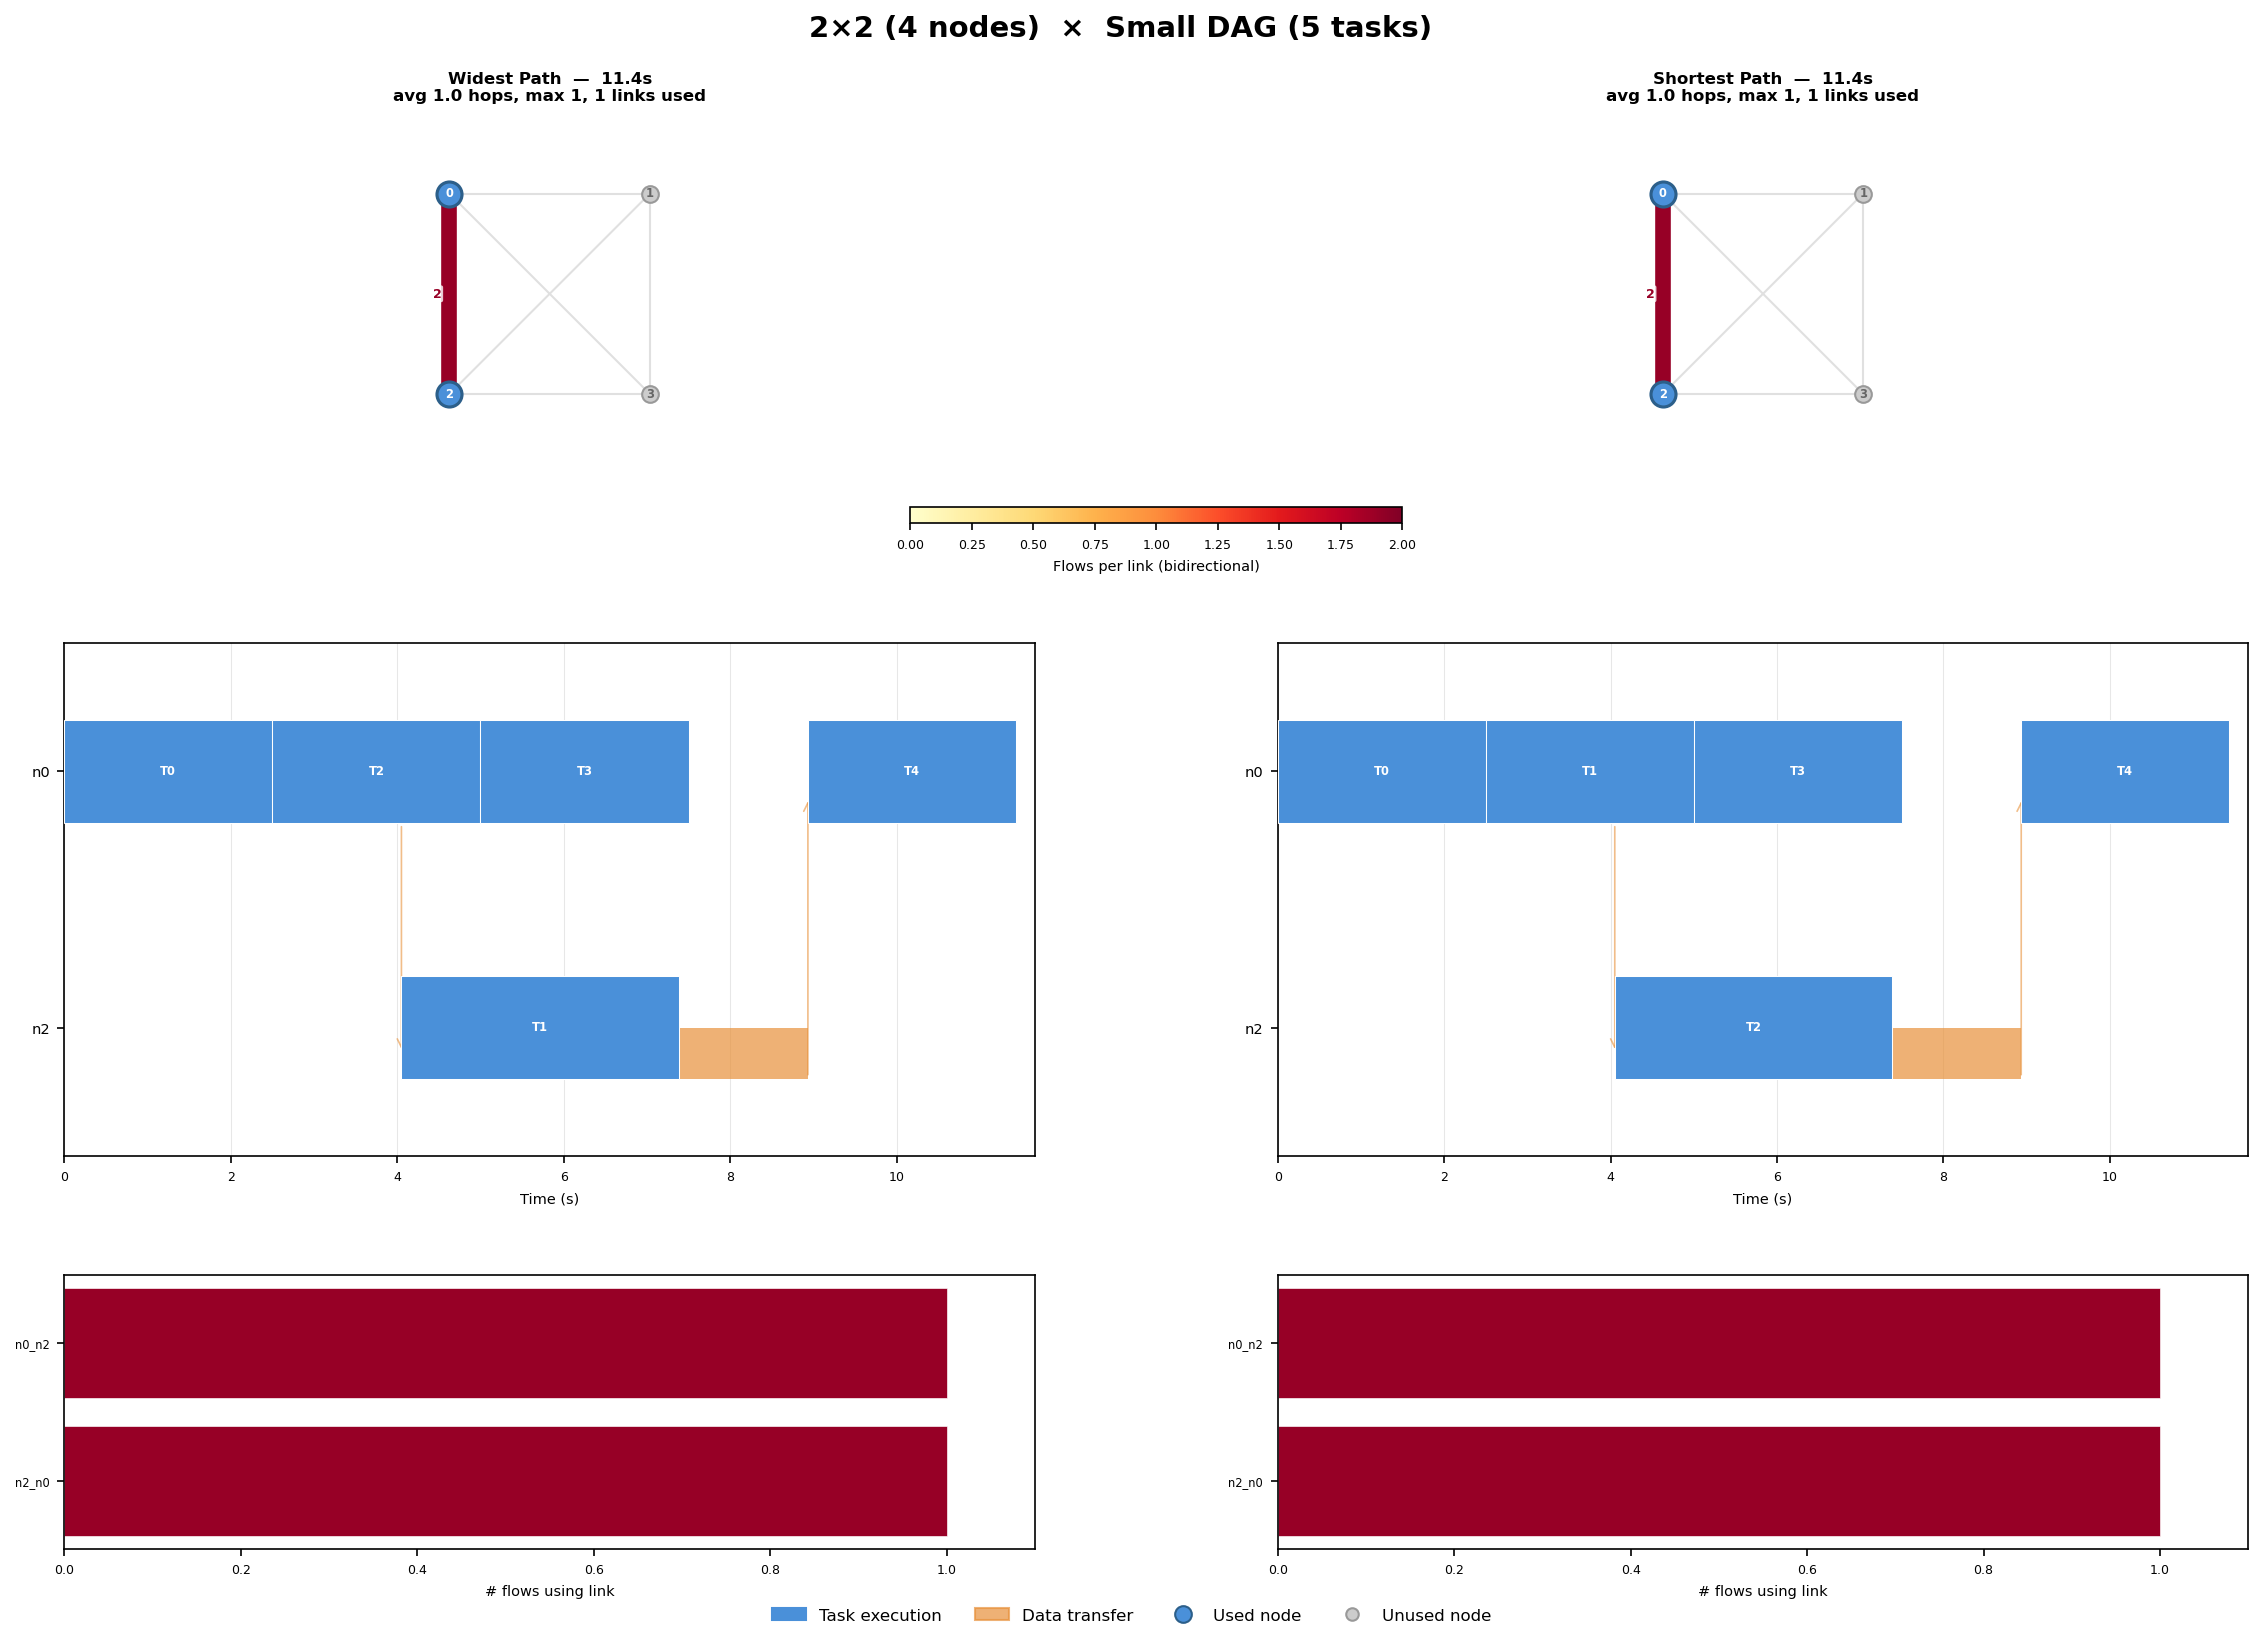
\includegraphics[width=\textwidth]{figures/smallnet_smalldag.png}
\caption{$2\times2$ $\times$ Small DAG. Both routing strategies produce identical results.}
\label{fig:ss}
\end{figure}

With only 4 nodes and a simple fork-join DAG, HEFT places 4 of 5 tasks on the
fastest node (n0, capacity=200) and sends one task to n2. Both strategies use
the same single-hop direct link (n0$\leftrightarrow$n2) for both transfers.
There is no routing decision to make: the network is too small for path
diversity.

%% --- 2x2 Medium ---
\subsection{$2\times2$ Network $\times$ Medium DAG (10 tasks)}

\begin{figure}[h]
\centering
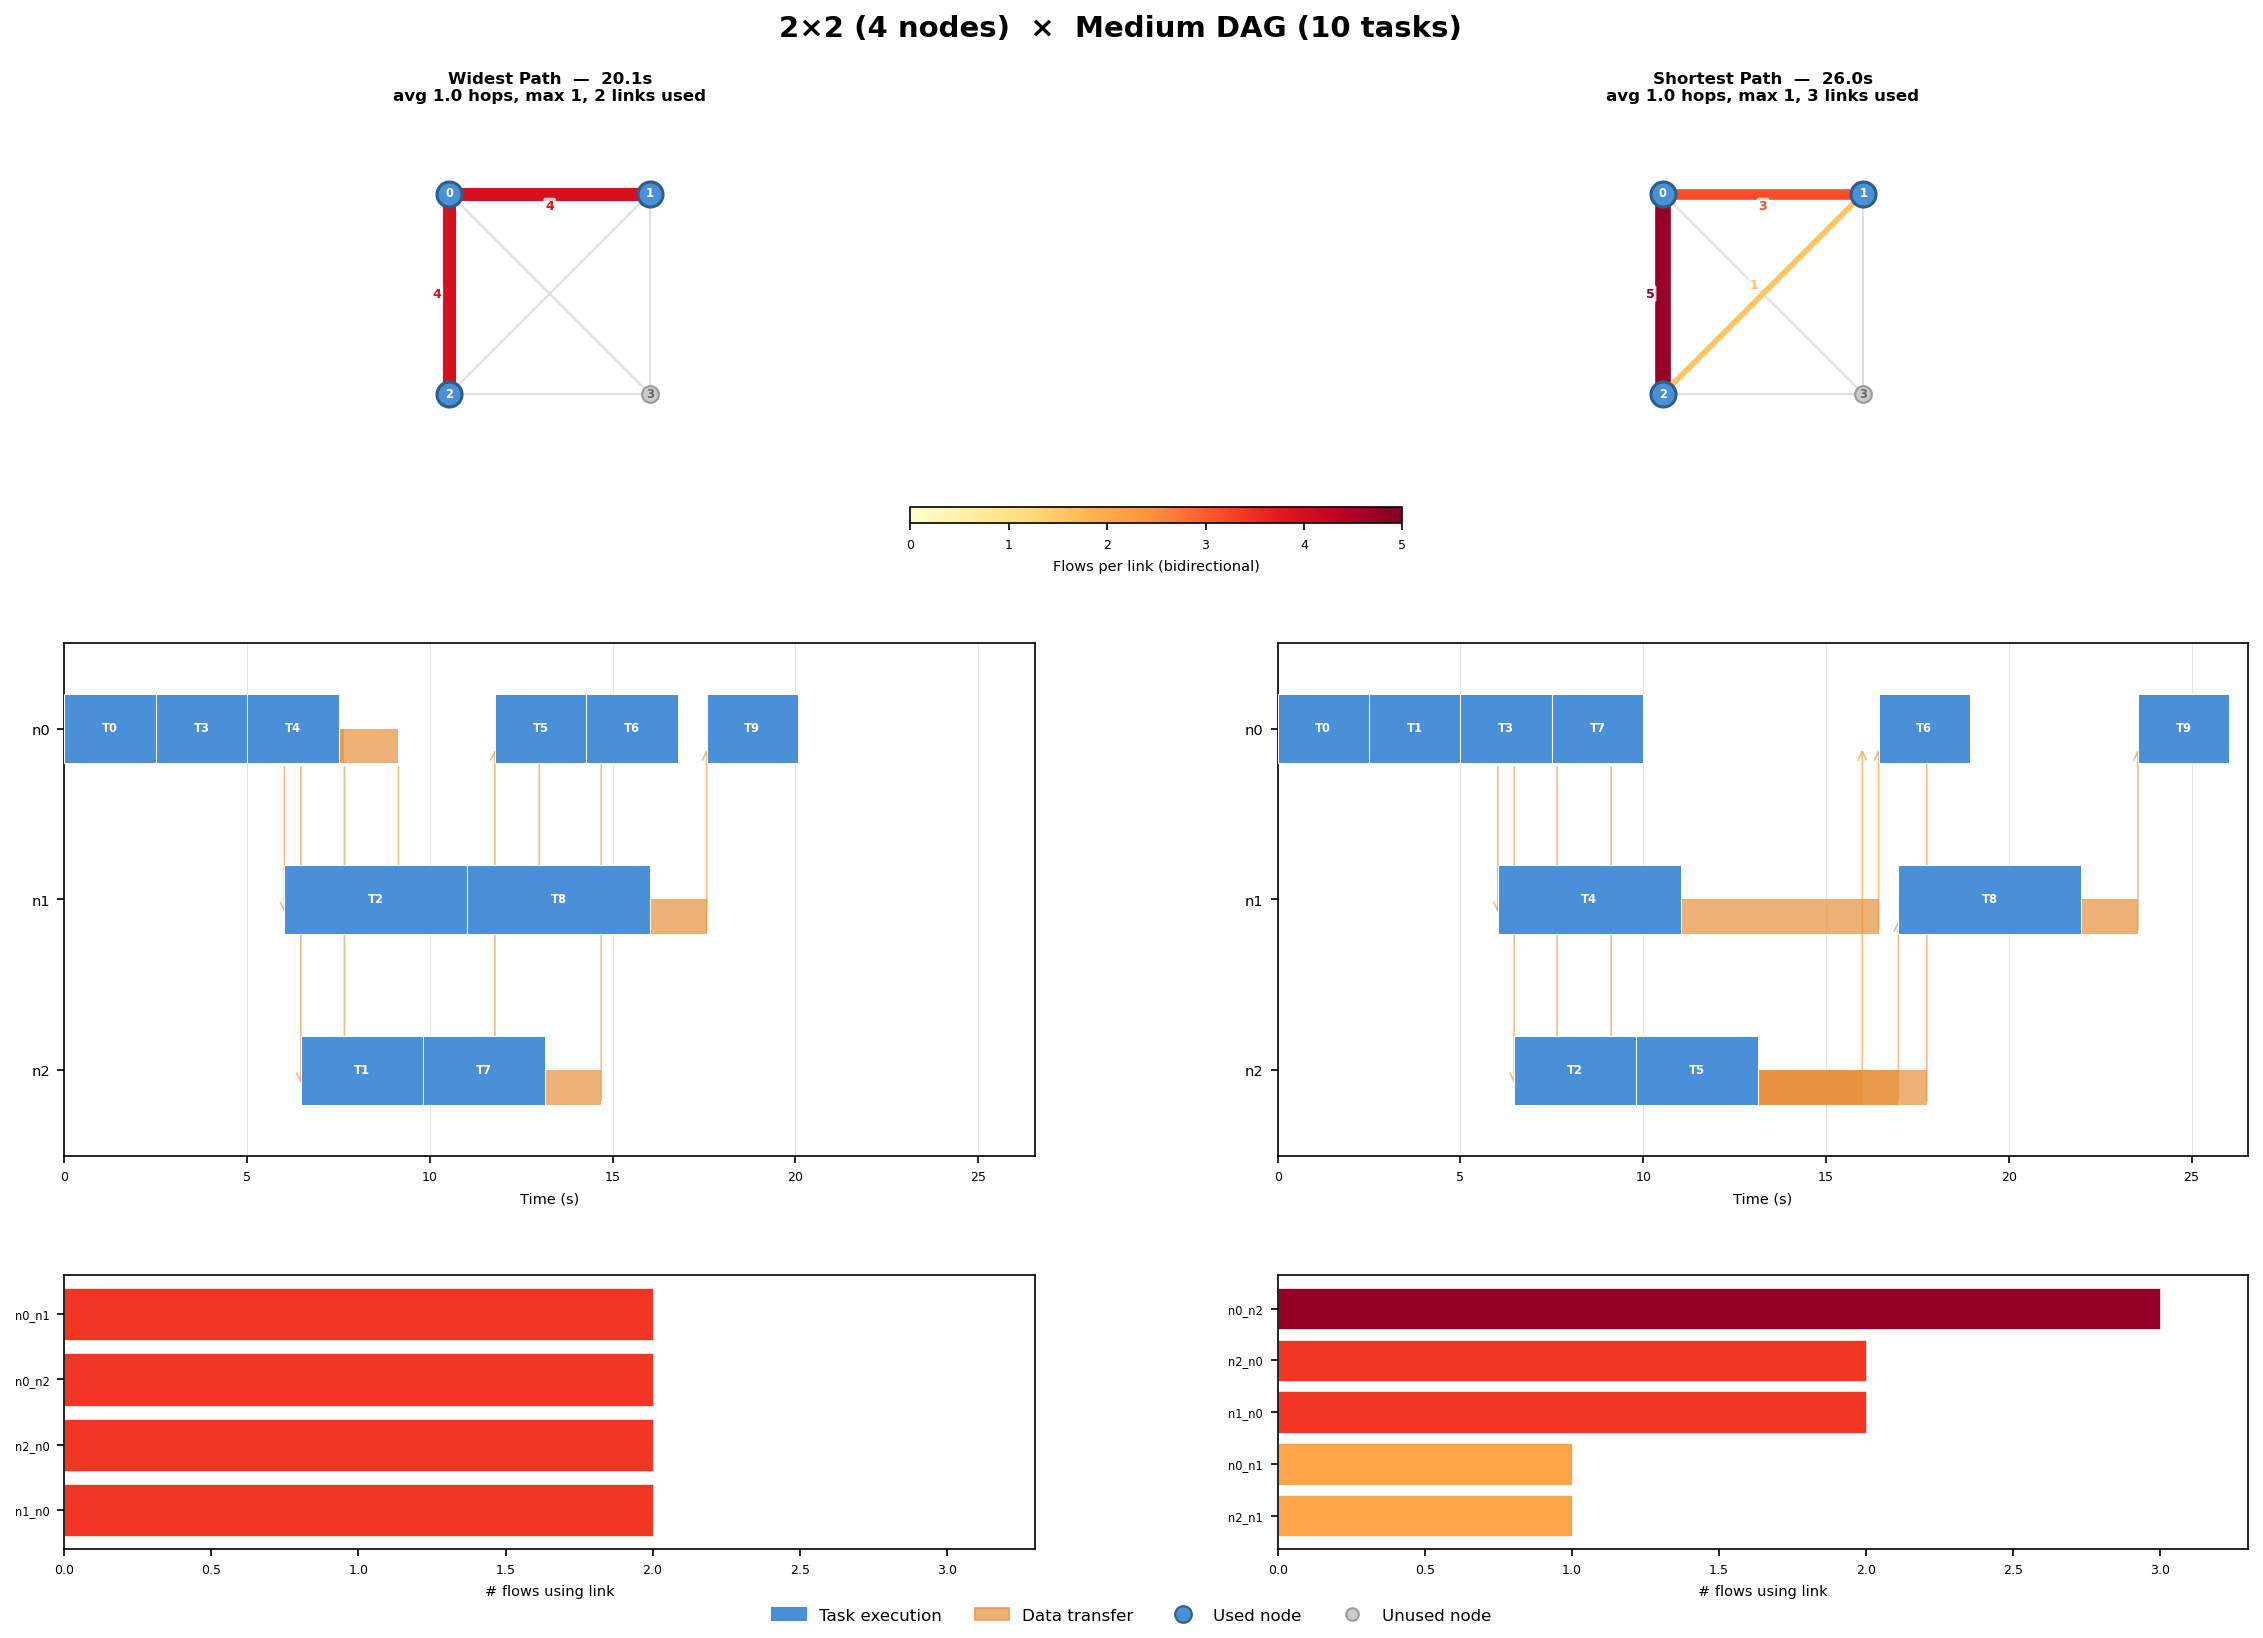
\includegraphics[width=\textwidth]{figures/smallnet_mediumdag.png}
\caption{$2\times2$ $\times$ Medium DAG. Widest path wins by balancing load across two links.}
\label{fig:sm}
\end{figure}

This is the \emph{only case where widest-path wins}. With 10 tasks across
3~nodes, widest path distributes 8 transfers evenly: 2 flows each on the four
directed links (n0$\to$n1, n0$\to$n2, n2$\to$n0, n1$\to$n0). Shortest path
concentrates 3 flows onto n0$\to$n2 while underusing other links. In a tiny
network where all links have the same hop count, widest-path's bandwidth
preference accidentally acts as a load balancer.

%% --- 2x2 Large ---
\subsection{$2\times2$ Network $\times$ Large DAG (20 tasks)}

\begin{figure}[h]
\centering
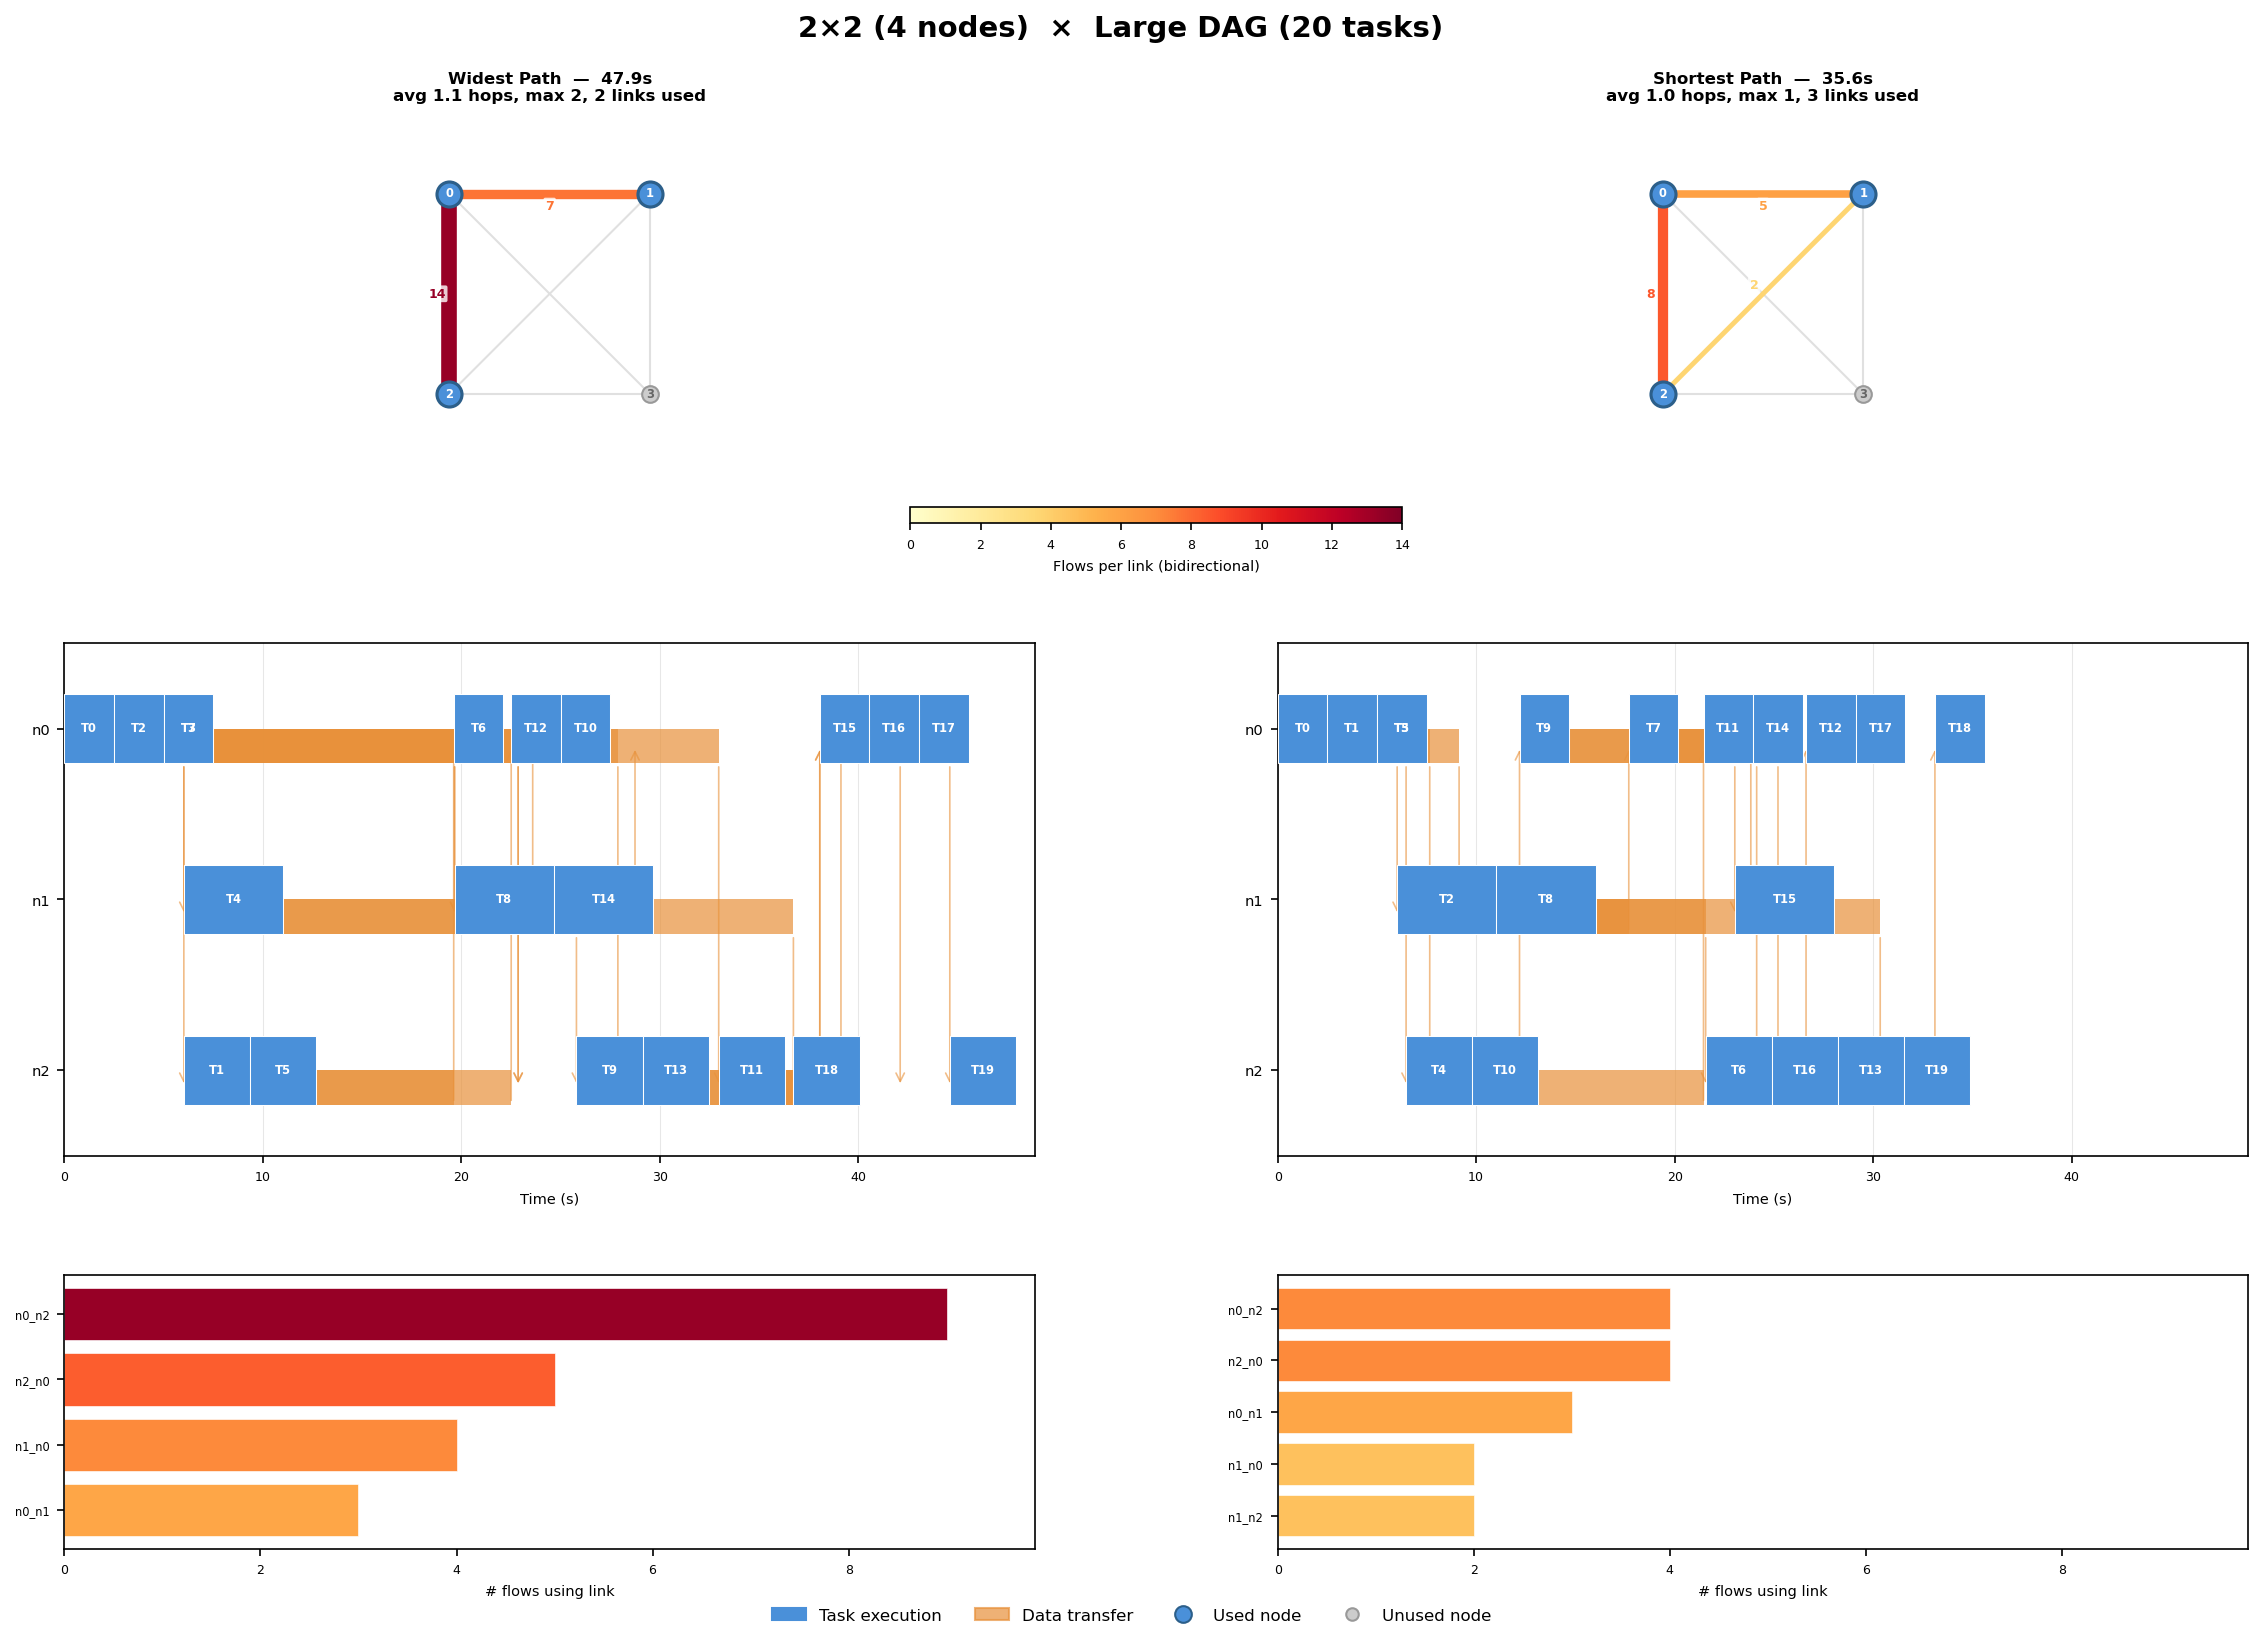
\includegraphics[width=\textwidth]{figures/smallnet_largedag.png}
\caption{$2\times2$ $\times$ Large DAG. Widest path concentrates 14 flows on link n0--n2.}
\label{fig:sl}
\end{figure}

With 20 tasks on 3 nodes, the flow-concentration problem emerges. The topology
panel shows widest path piling \textbf{14 bidirectional flows} onto the
n0$\leftrightarrow$n2 link (thick dark red), while the n0$\leftrightarrow$n1
link carries only 7 (thinner orange). Widest path also introduces 2-hop
routes, doubling link occupancy per transfer. Shortest path distributes
traffic more evenly across 3 physical links (max 8 flows), with all transfers
using direct 1-hop routes. The Gantt chart shows widest path's transfers
stretching to $\sim$45\,s while shortest path finishes by 35.6\,s.

%% --- 3x3 Small ---
\subsection{$3\times3$ Network $\times$ Small DAG (5 tasks)}

\begin{figure}[h]
\centering
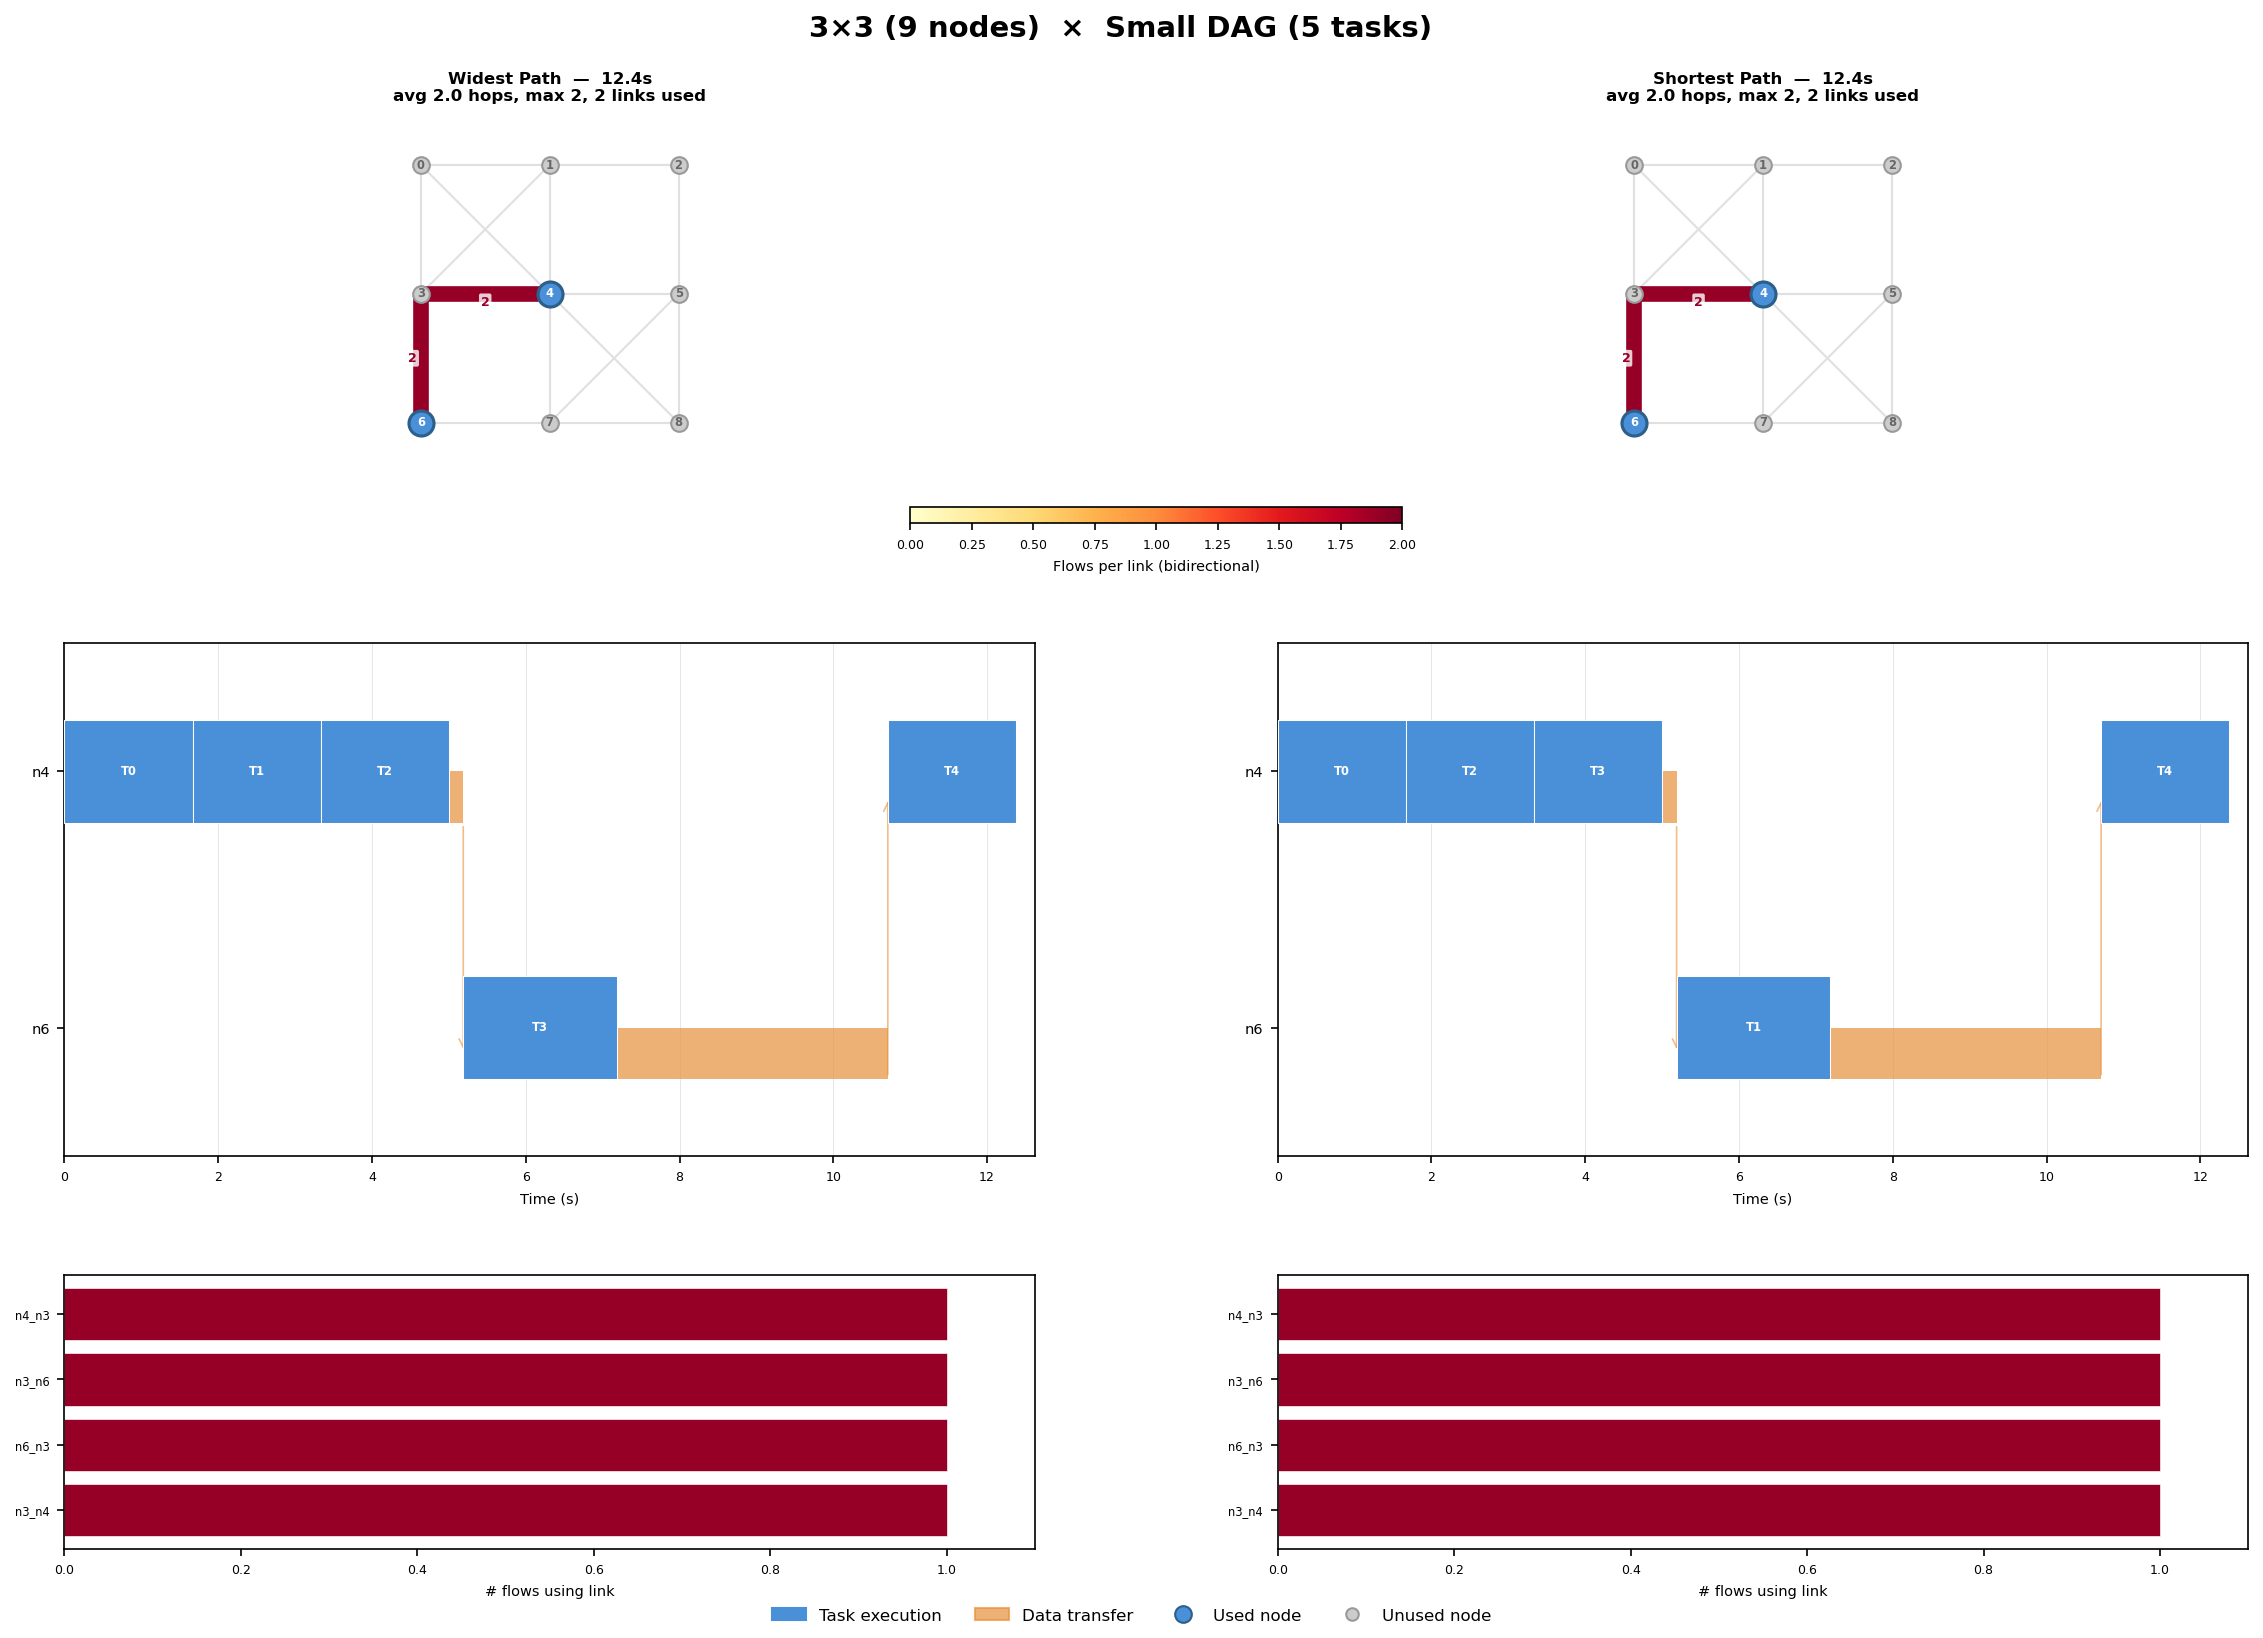
\includegraphics[width=\textwidth]{figures/mediumnet_smalldag.png}
\caption{$3\times3$ $\times$ Small DAG. Both strategies take the same 2-hop path through n3.}
\label{fig:ms}
\end{figure}

HEFT concentrates 4 of 5 tasks on n4 (center, capacity=300) and places one
task on a corner node. Both strategies must traverse the same 2-hop path
(n4$\to$n3$\to$n6 and back). With only 2 sequential transfers and no
alternative paths, routing is irrelevant.

%% --- 3x3 Medium ---
\subsection{$3\times3$ Network $\times$ Medium DAG (10 tasks)}

\begin{figure}[h]
\centering
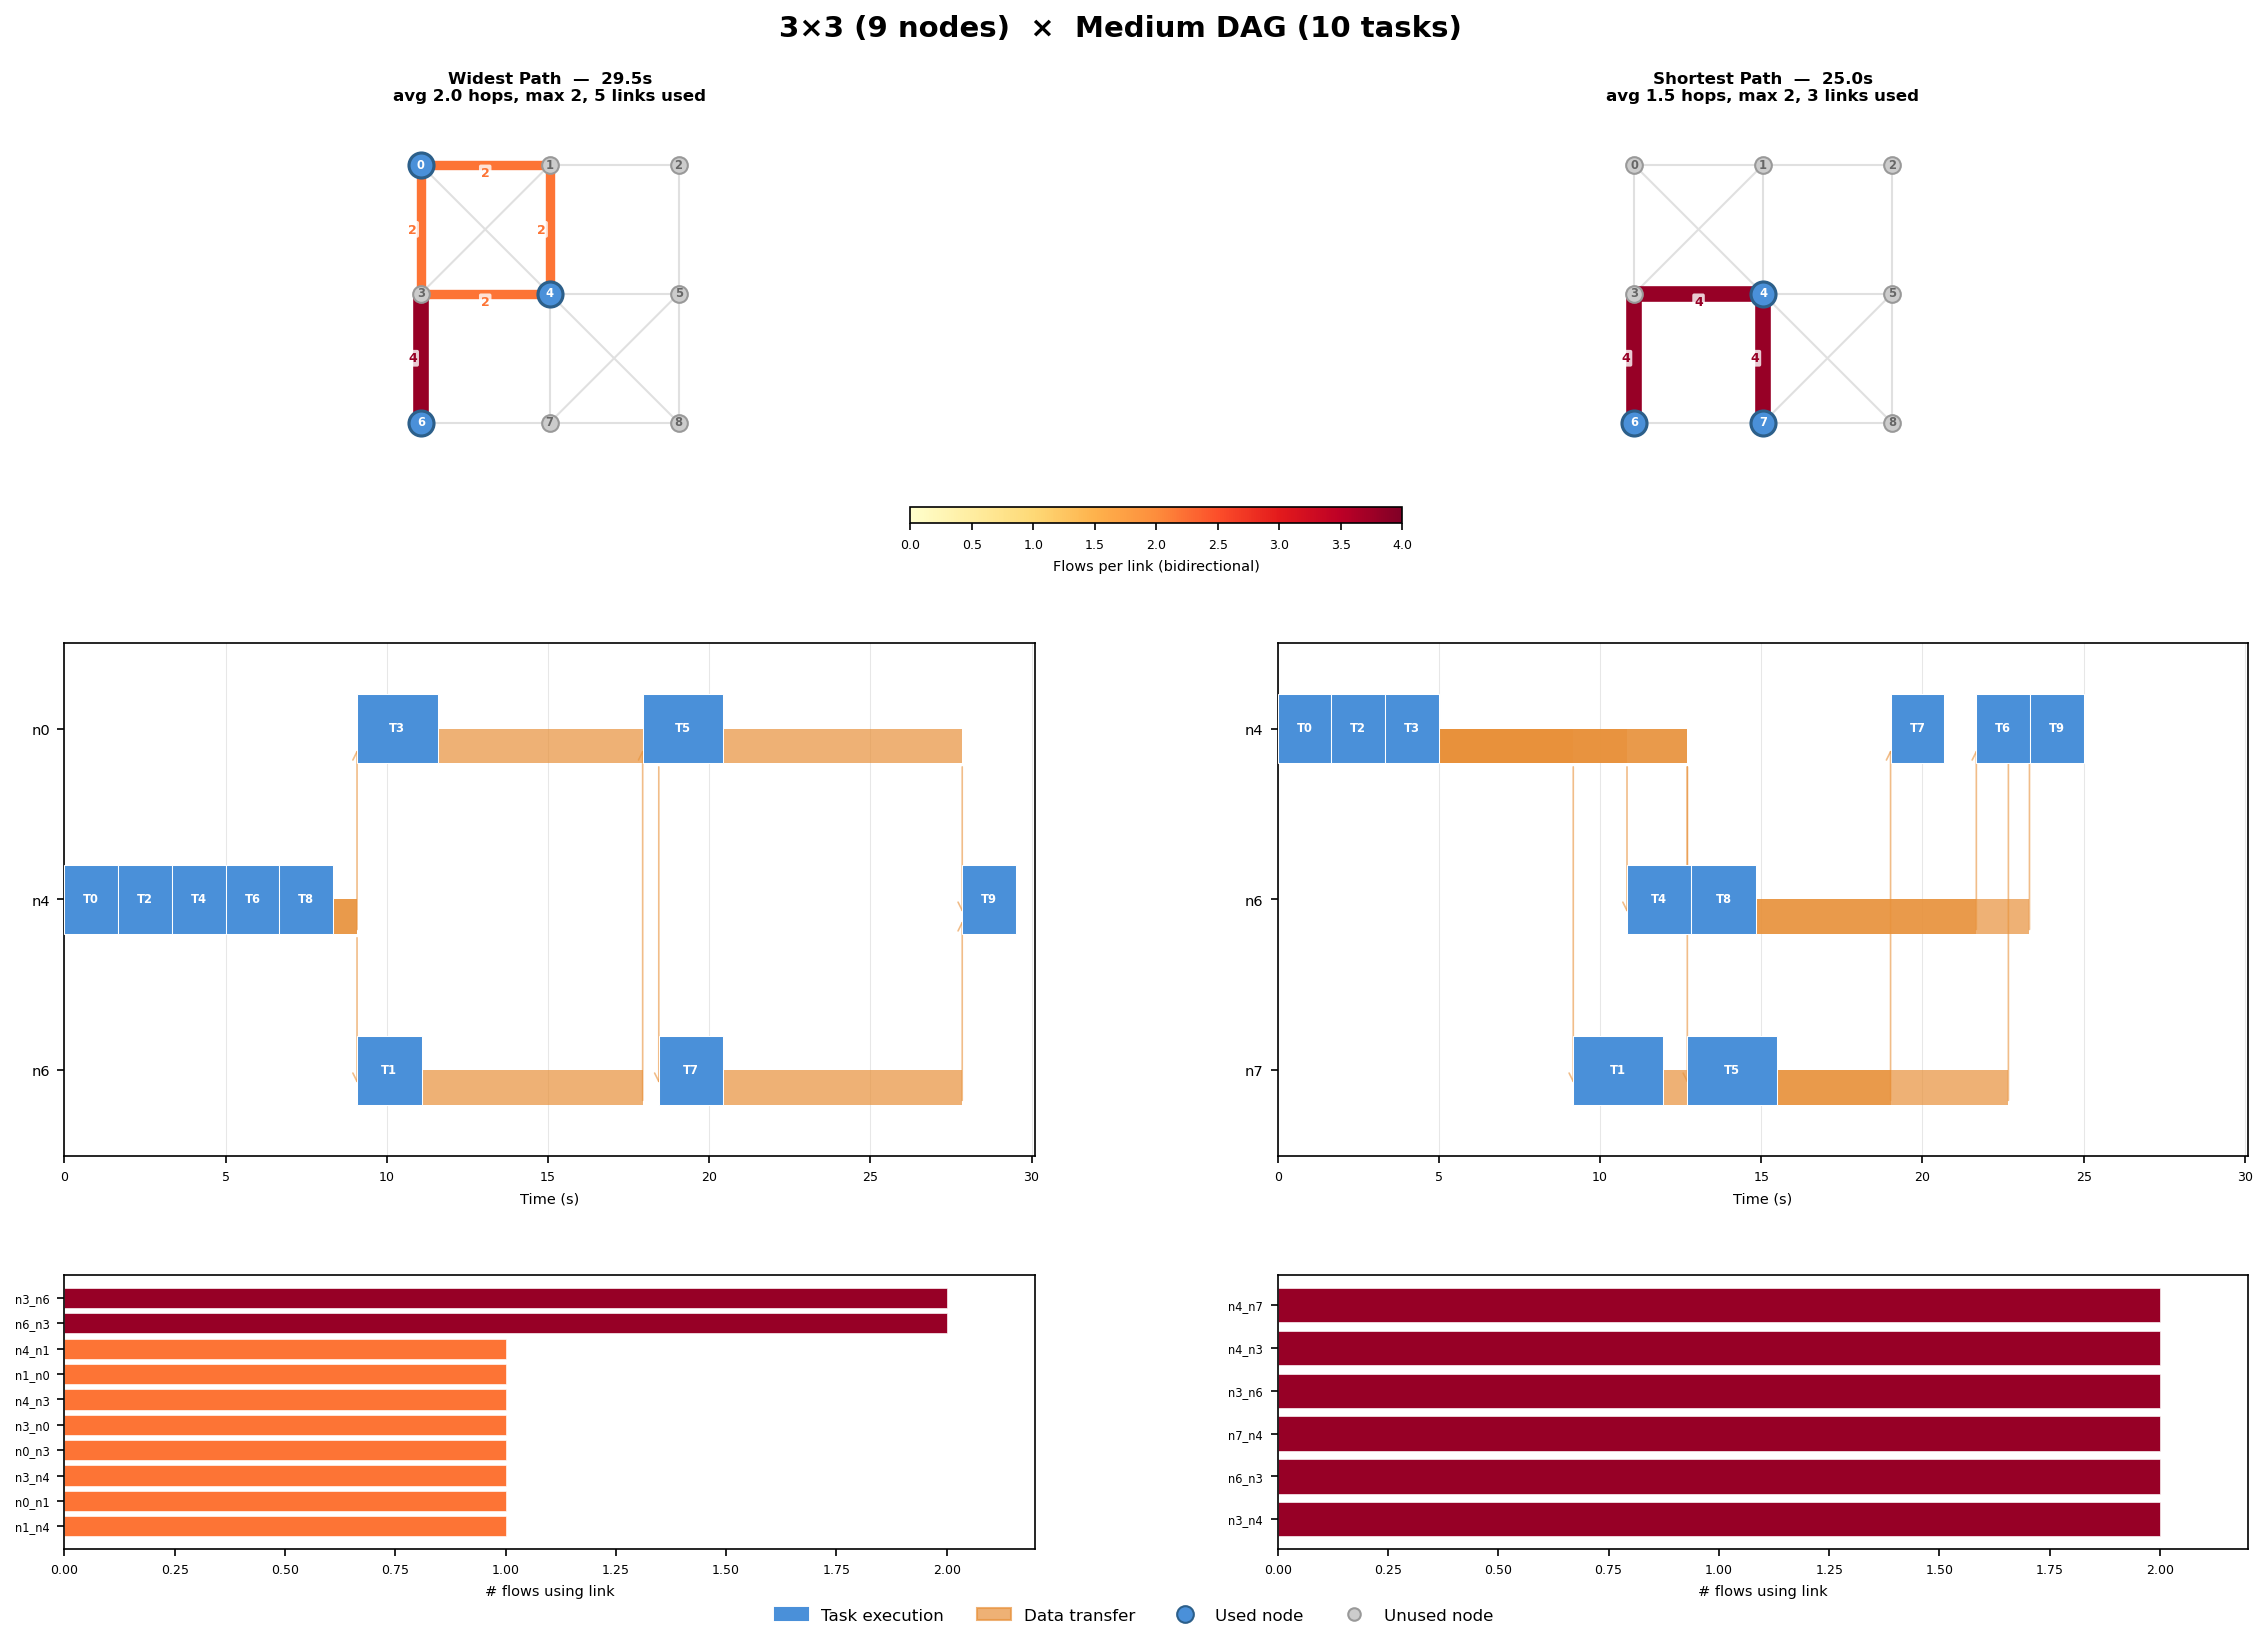
\includegraphics[width=\textwidth]{figures/mediumnet_mediumdag.png}
\caption{$3\times3$ $\times$ Medium DAG. Widest path scatters traffic through n0 and n6
via 10 different links; shortest path uses 6 links concentrated around n4's neighbors.}
\label{fig:mm}
\end{figure}

The topology panels diverge clearly. Widest path routes traffic through
distant nodes (n0 and n6) via 2-hop paths through n1 and n3, activating
\textbf{10 unique links}. Shortest path concentrates on n4's direct neighbors
(n7 and n6) using only \textbf{6 unique links} with a lower average hop count
(1.5 vs.\ 2.0). Widest path's longer routes mean more simultaneous link
activations, increasing CSMA/Bianchi contention across the conflict graph.
Shortest path finishes 18\% faster.

%% --- 3x3 Large ---
\subsection{$3\times3$ Network $\times$ Large DAG (20 tasks)}

\begin{figure}[h]
\centering
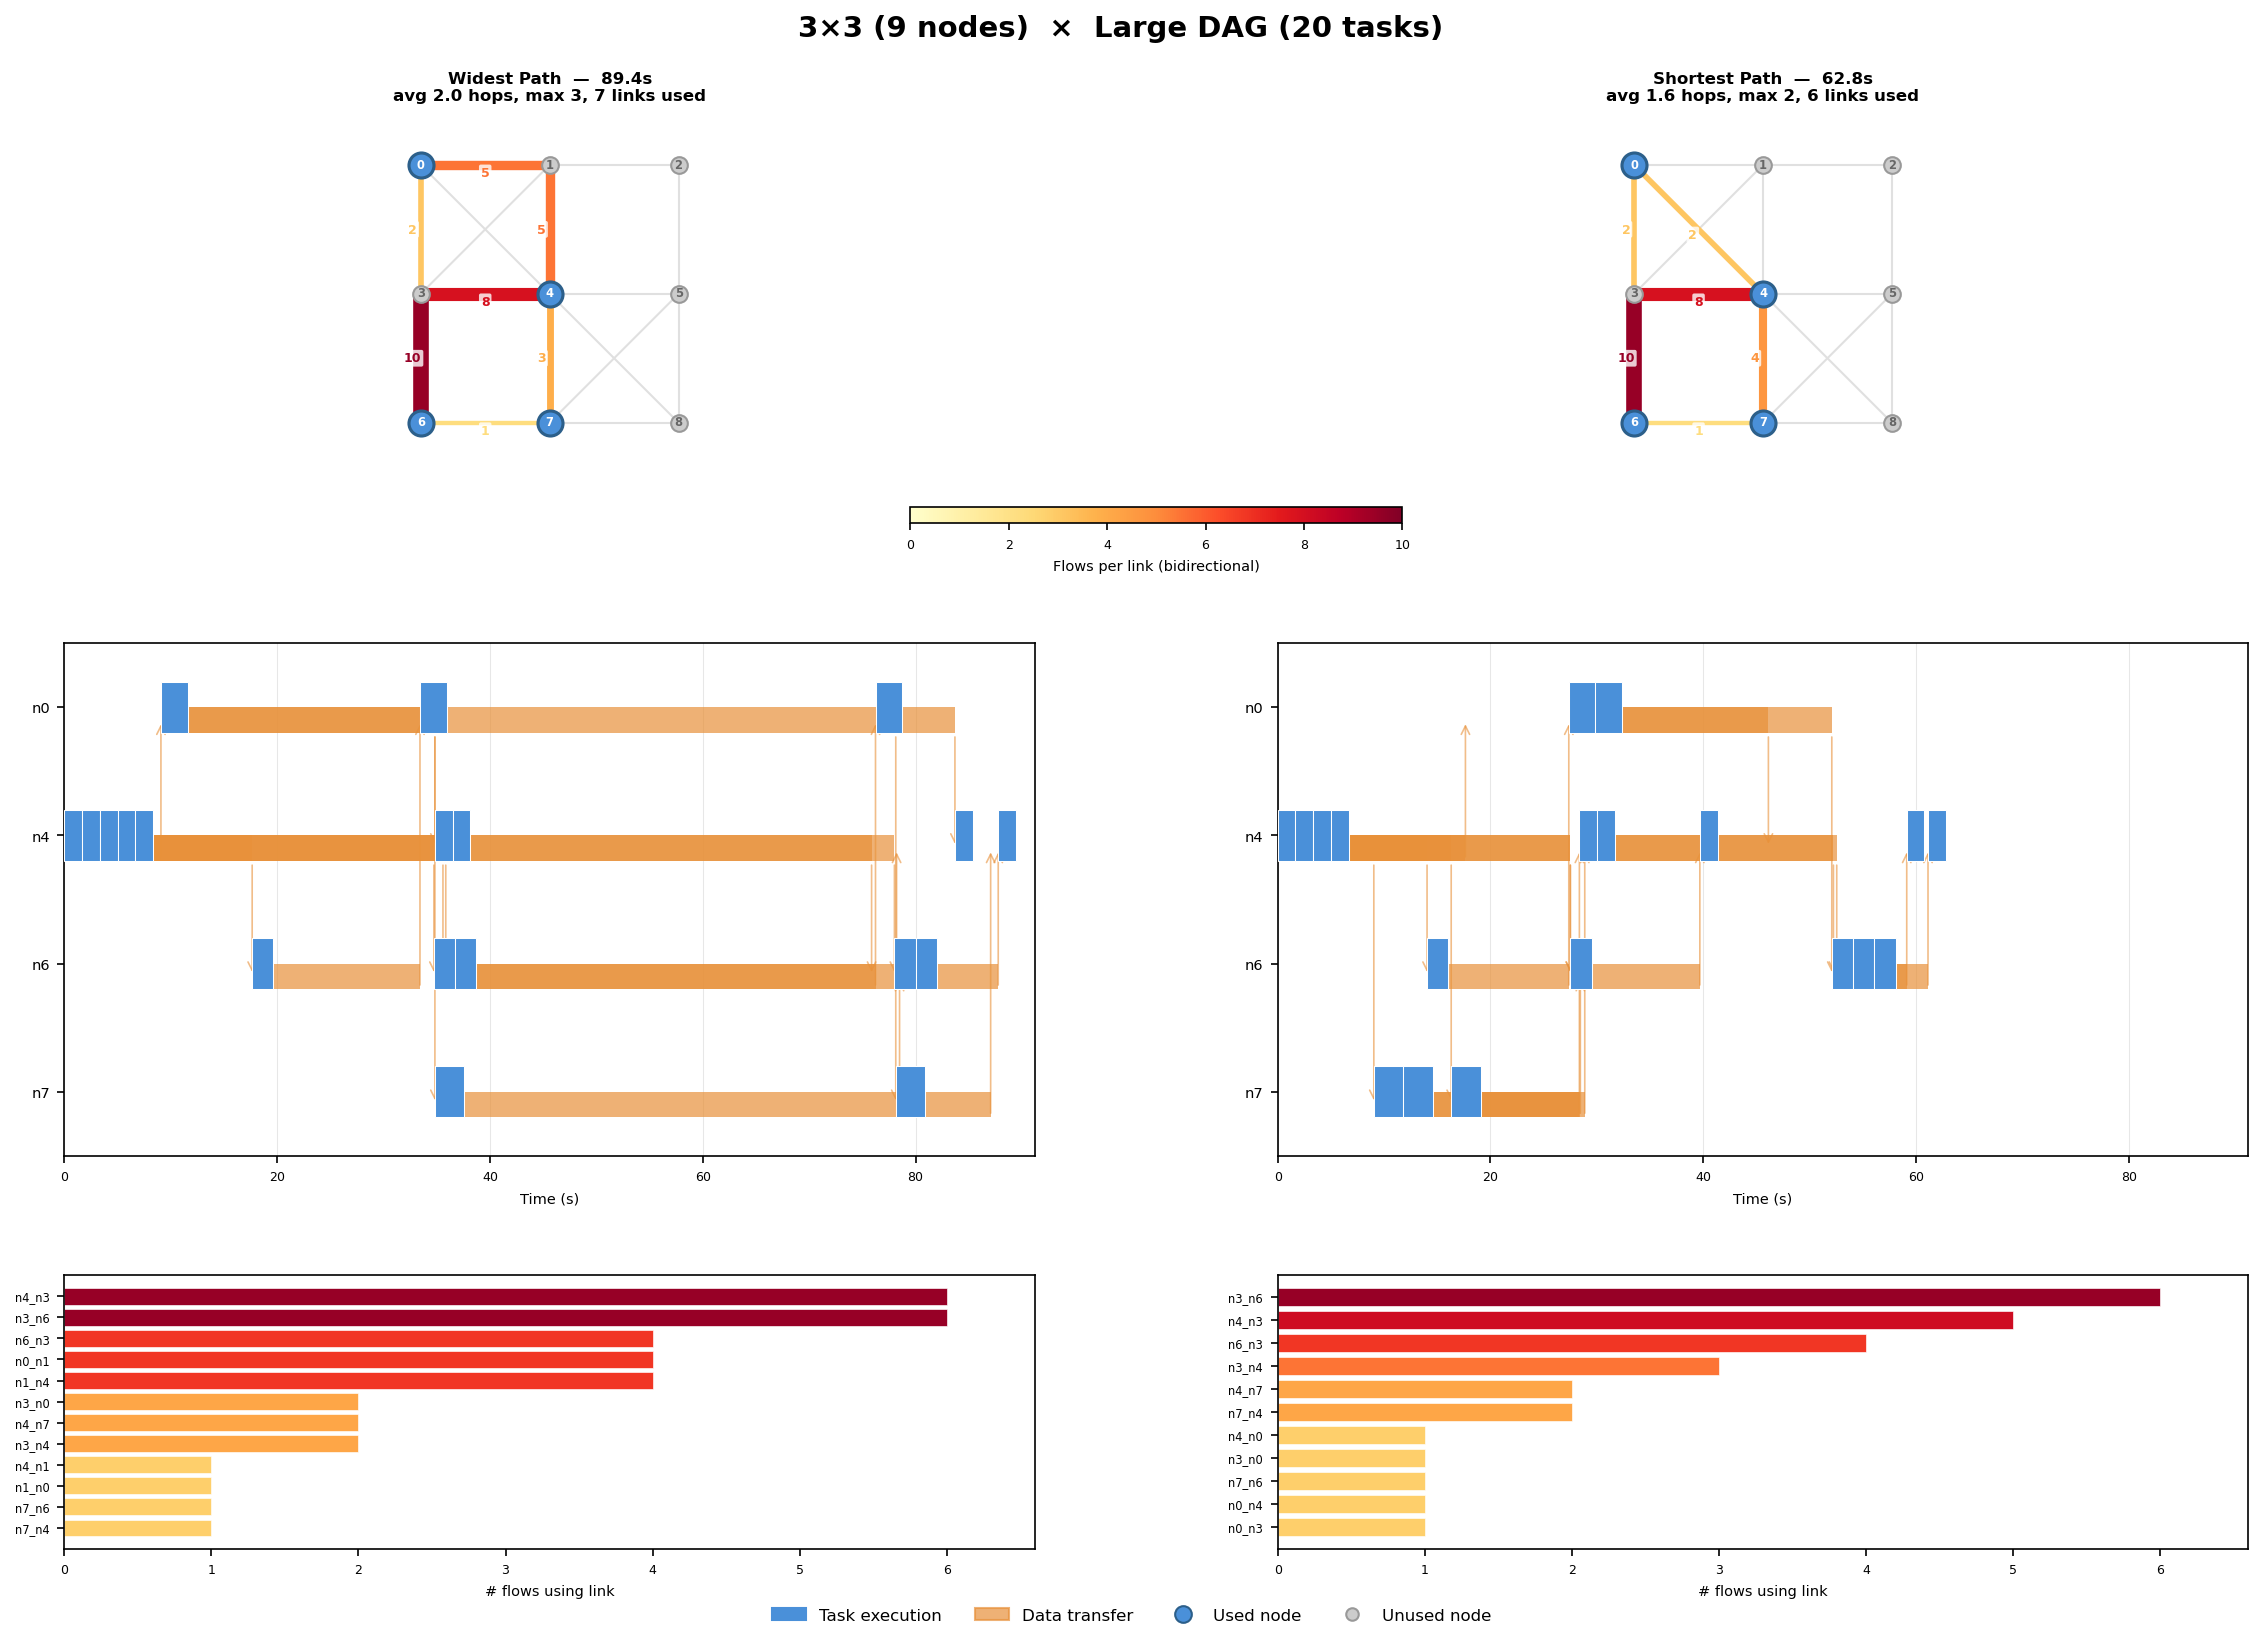
\includegraphics[width=\textwidth]{figures/mediumnet_largedag.png}
\caption{$3\times3$ $\times$ Large DAG. Widest path creates a congested n4--n3--n6 corridor
with 6 flows per link; some transfers include 3-hop routes.}
\label{fig:ml}
\end{figure}

With 20 tasks distributed across 4 nodes, widest path creates a heavily
loaded corridor: \textbf{6 flows each} on n4$\to$n3 and n3$\to$n6, plus 4
flows on n0$\to$n1 and n1$\to$n4. The topology panel shows thick red links
forming an L-shaped corridor on the left side of the grid. Widest path also
uses 3-hop routes (avg 2.0 hops, max 3), tripling the link occupancy per
transfer. The Gantt chart shows n4 blocked by transfer activity from $t=5$ to
$t=78$\,s. Shortest path uses a similar number of unique links (6 vs.\ 7) but
with lower hop counts (avg 1.6, max 2), completing 42\% faster.

%% --- 4x4 Small ---
\subsection{$4\times4$ Network $\times$ Small DAG (5 tasks)}

\begin{figure}[h]
\centering
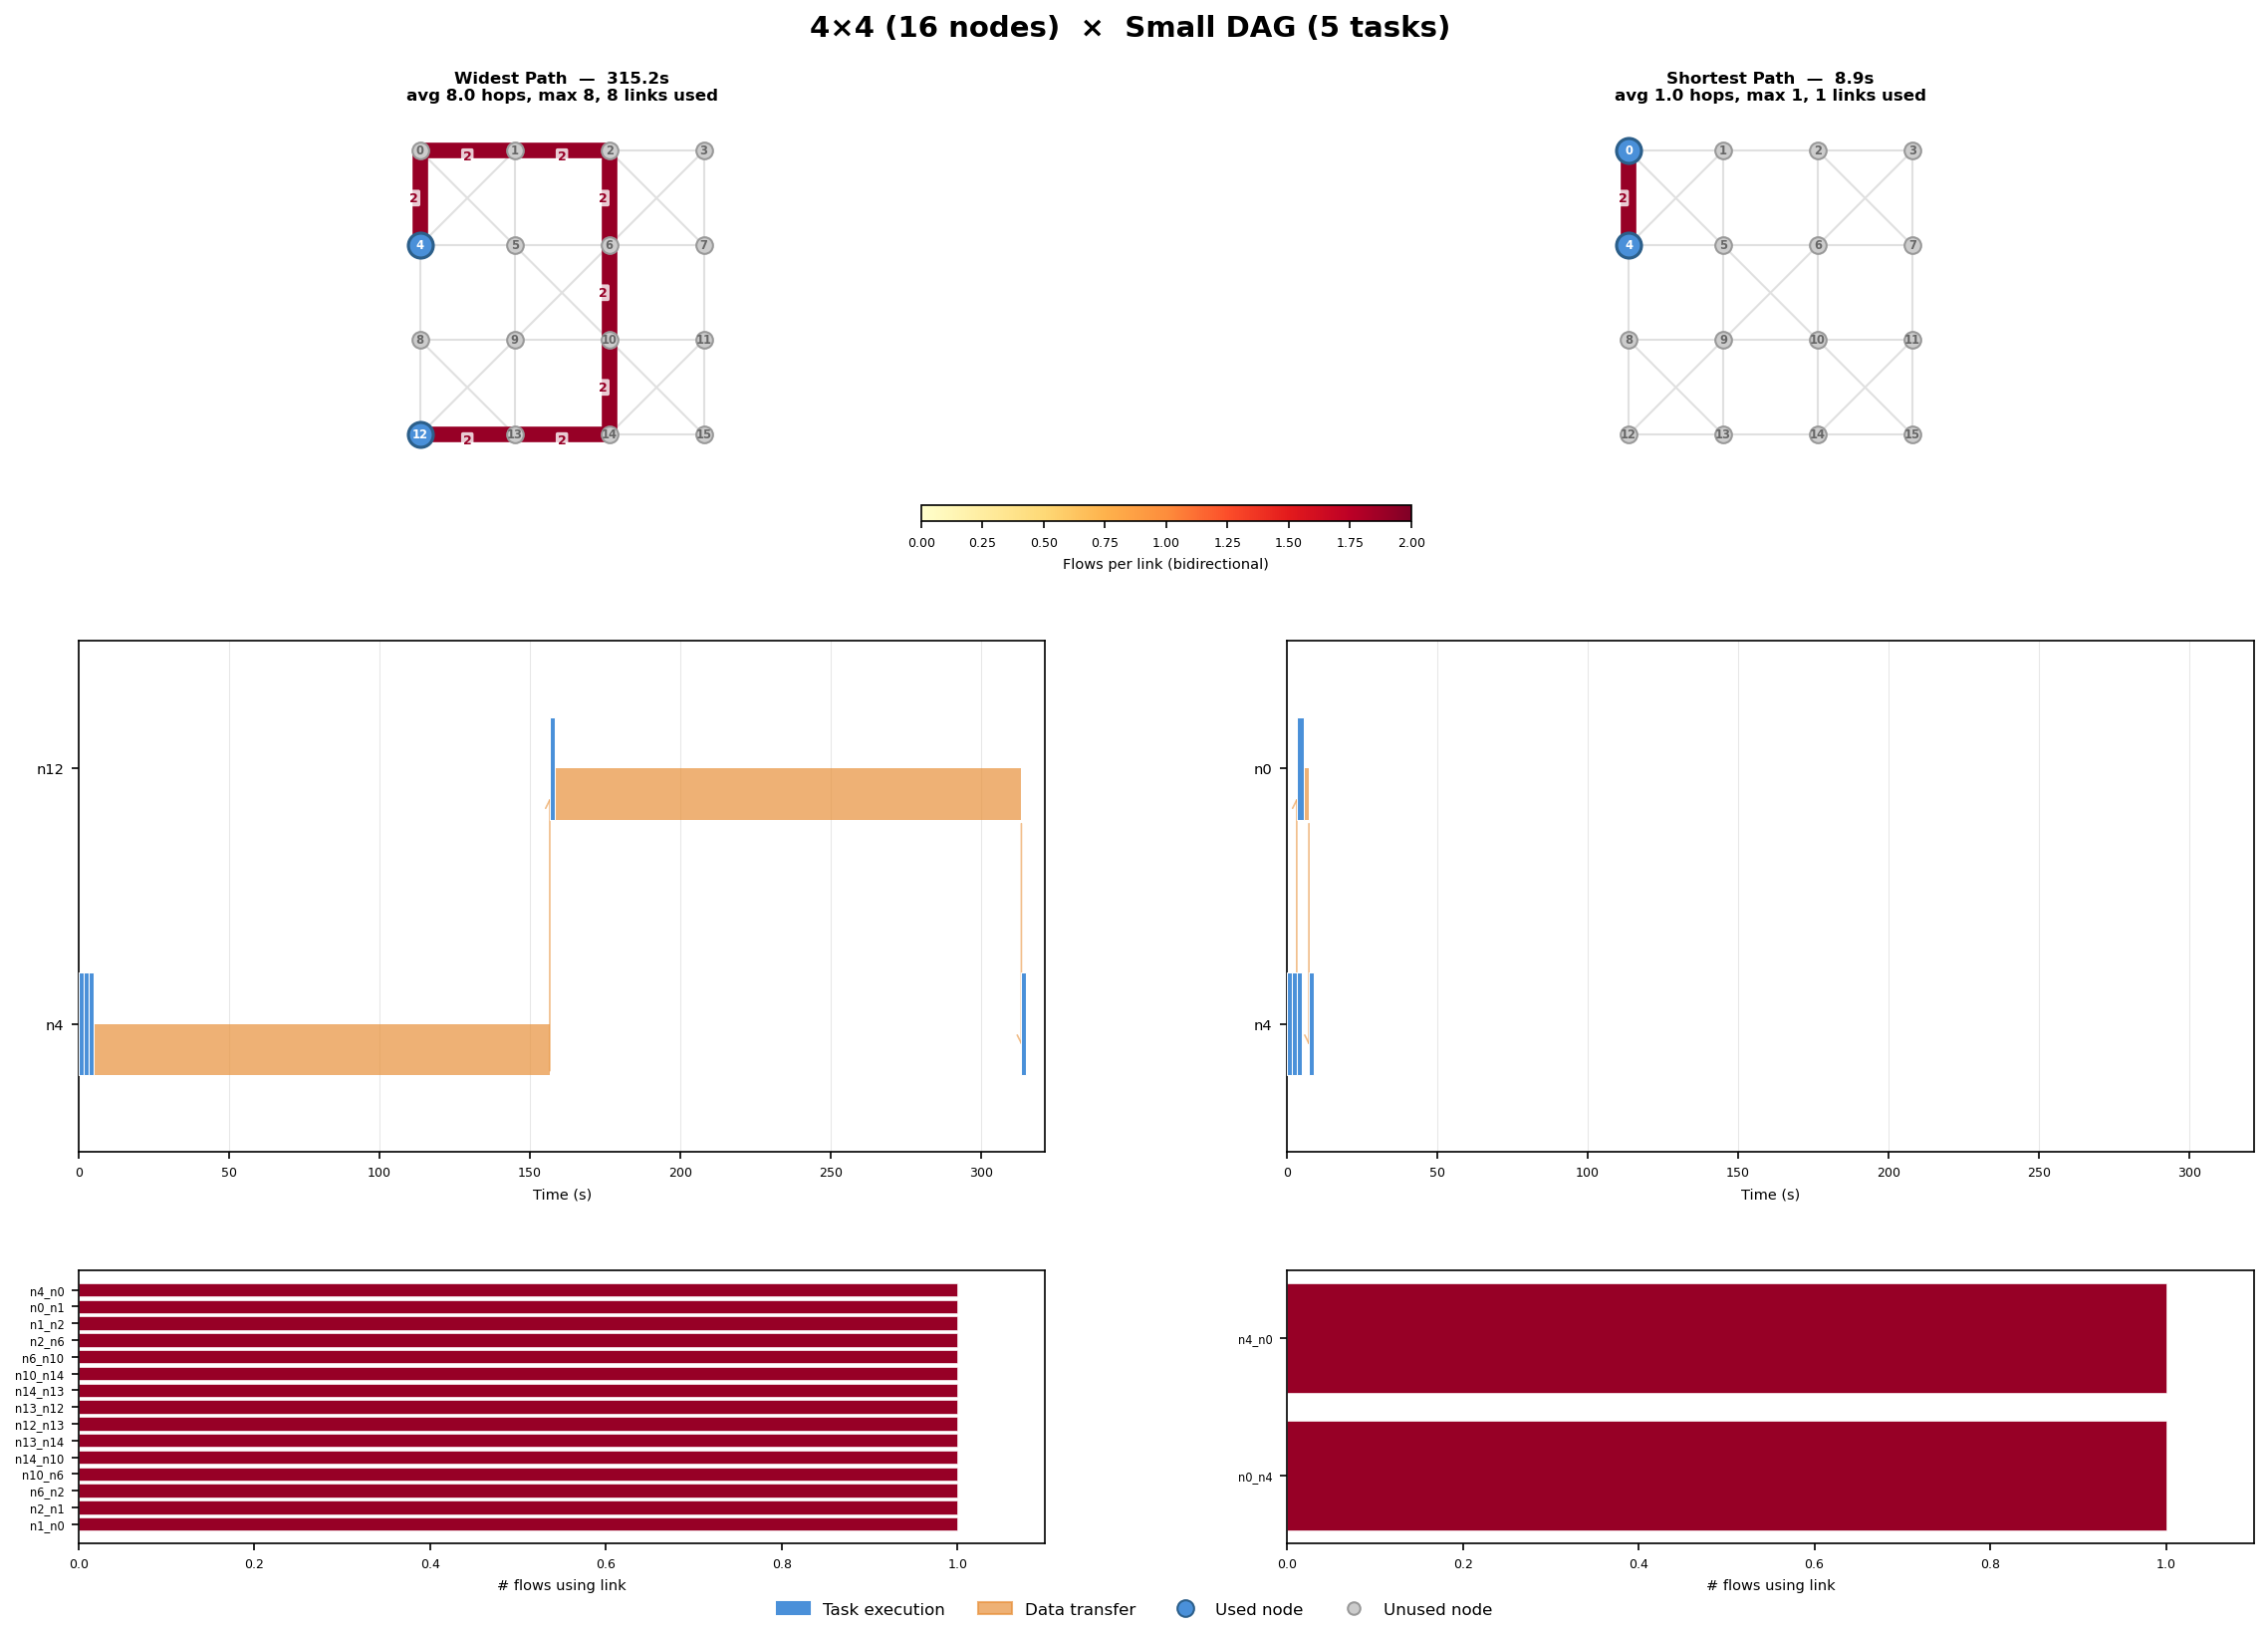
\includegraphics[width=\textwidth]{figures/largenet_smalldag.png}
\caption{$4\times4$ $\times$ Small DAG. Widest path takes an 8-hop perimeter route to n12;
shortest path uses a 1-hop direct link to n0. The $35\times$ slowdown is the most extreme case.}
\label{fig:ls}
\end{figure}

This is the most dramatic case. HEFT assigns one task to a remote node via
widest-path routing: the transfer traverses an \textbf{8-hop perimeter route}
(n4$\to$n0$\to$n1$\to$n2$\to$n6$\to$n10$\to$n14$\to$n13$\to$n12), taking
155\,s per direction. The topology panel shows all 8 links uniformly red.
Each hop adds latency, and with csma\_bianchi, each of the 8 links must
contend for airtime. In contrast, shortest path sends the task to the
adjacent node n0 via a \textbf{single 1-hop link}, completing in 1.5\,s. The
makespan ratio is $315.2 / 8.9 = 35.4\times$.

%% --- 4x4 Medium ---
\subsection{$4\times4$ Network $\times$ Medium DAG (10 tasks)}

\begin{figure}[h]
\centering
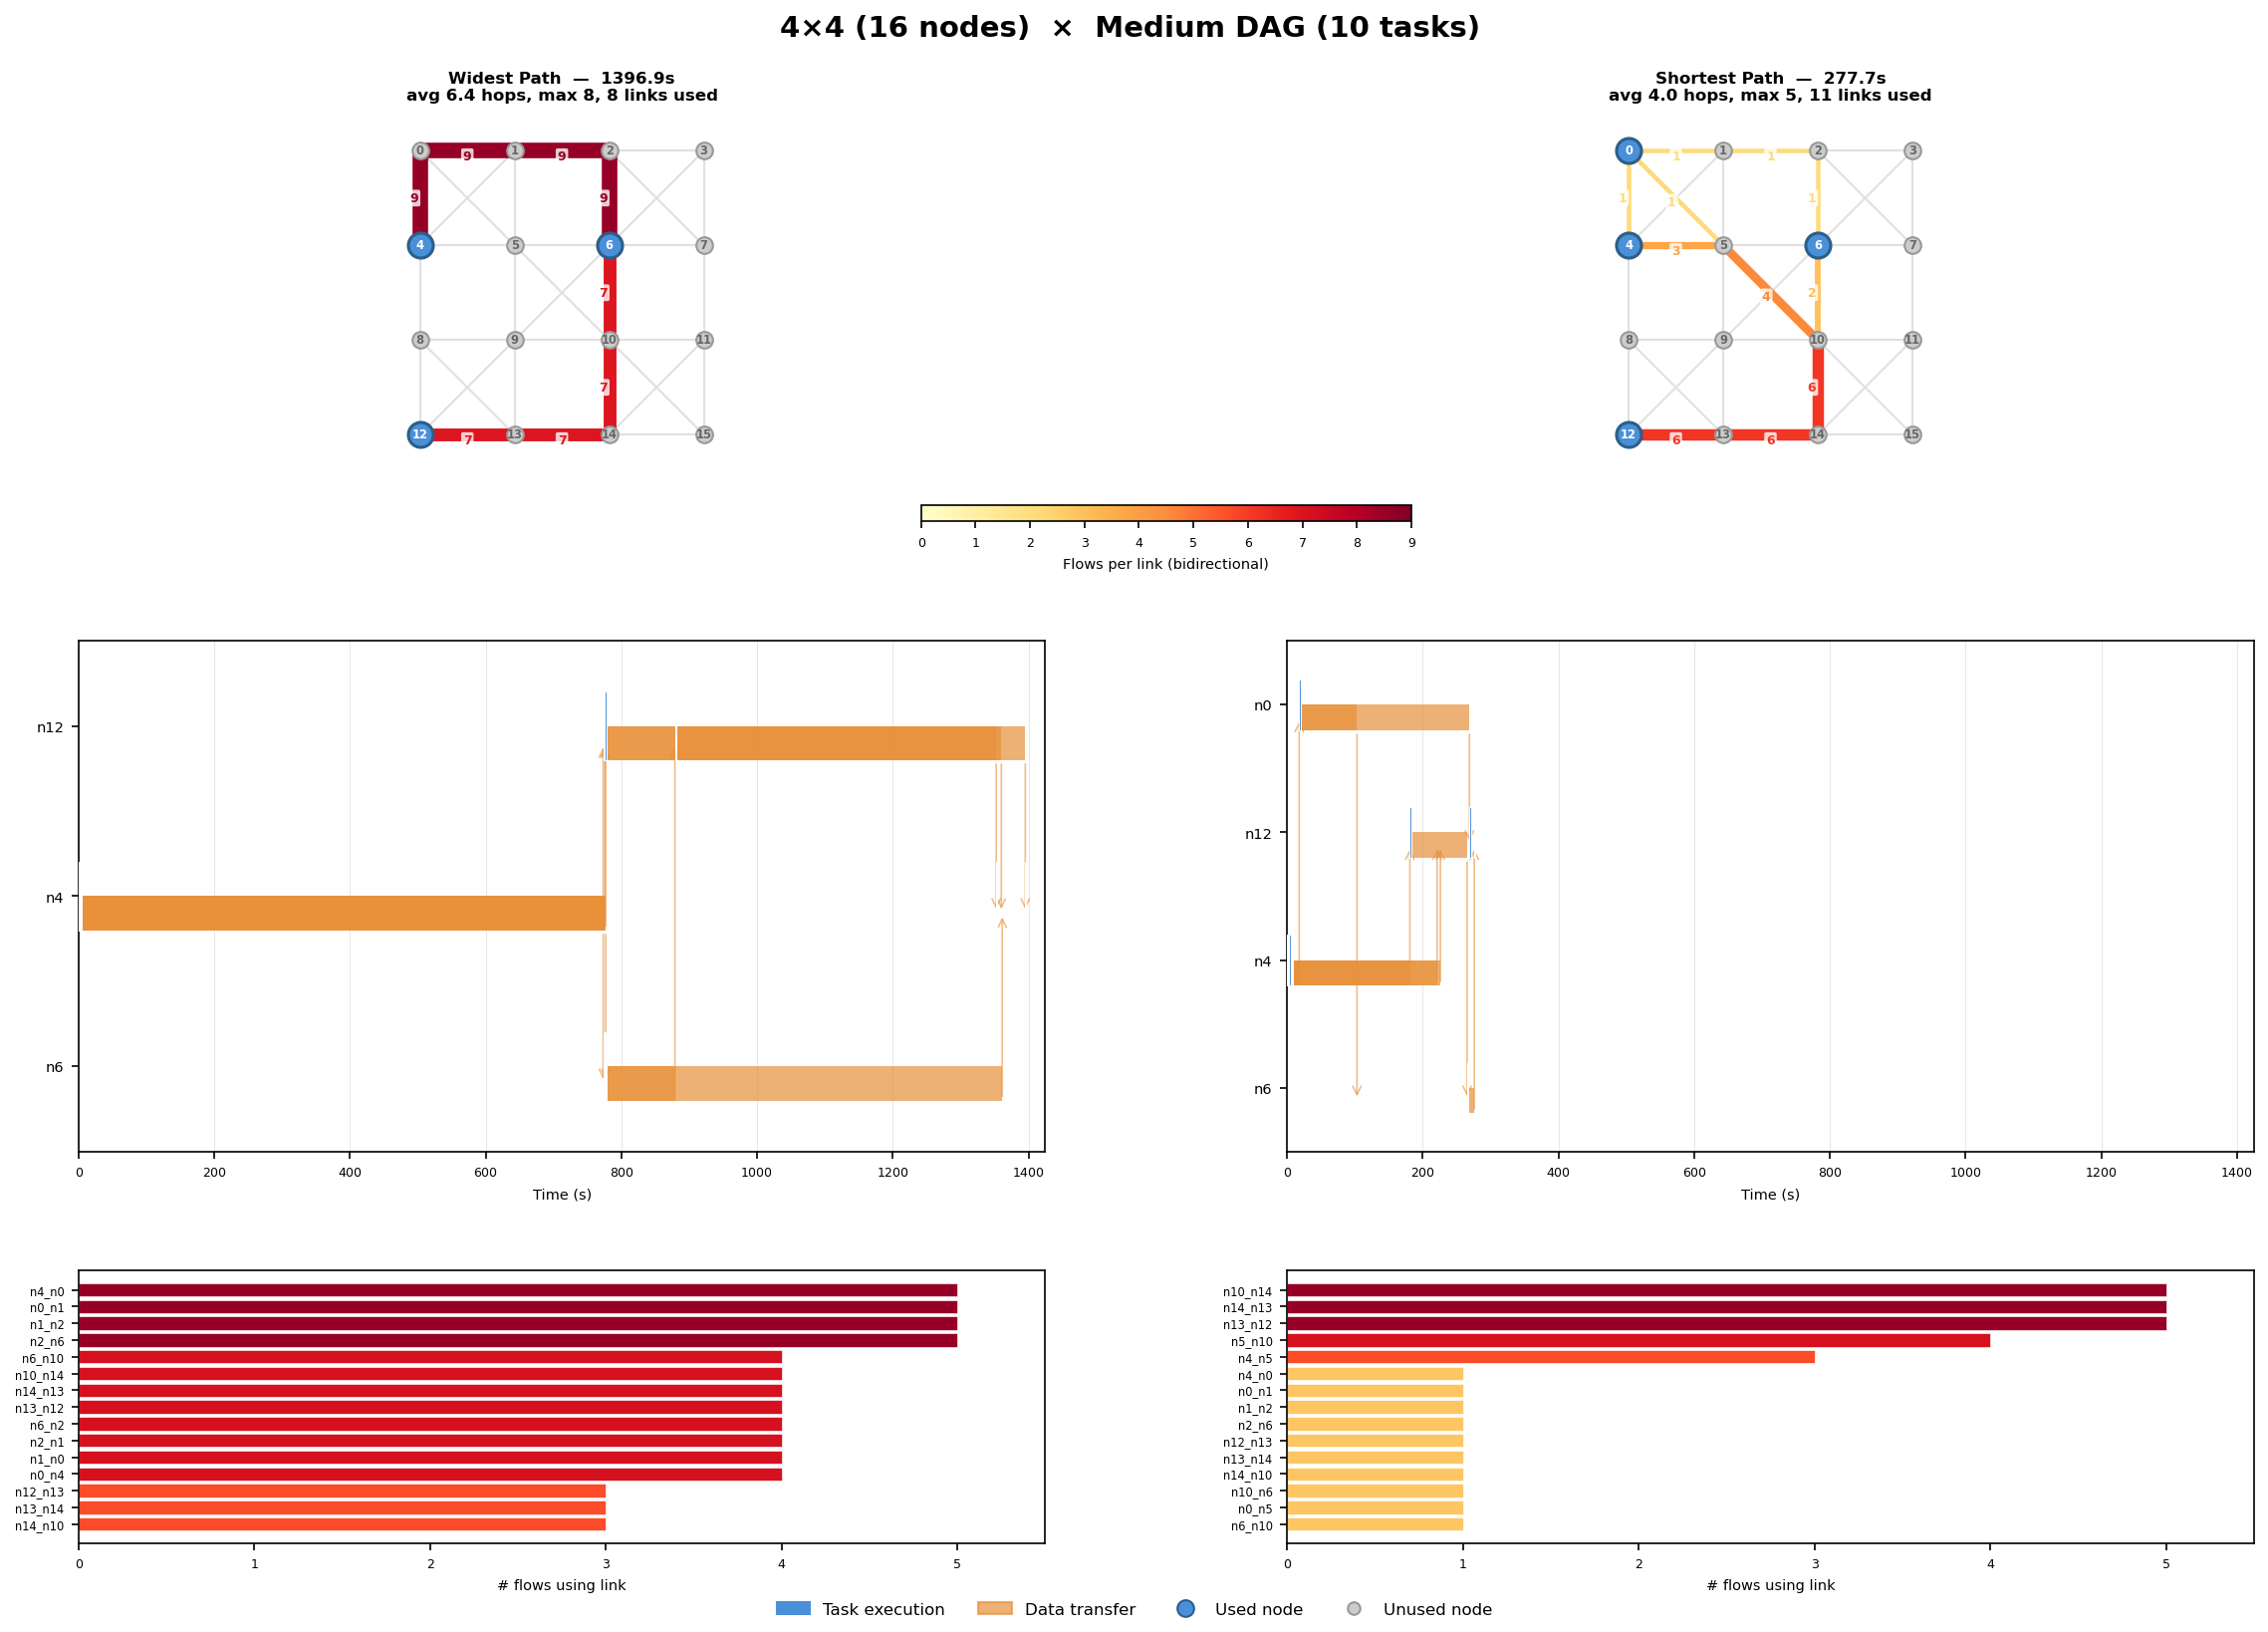
\includegraphics[width=\textwidth]{figures/largenet_mediumdag.png}
\caption{$4\times4$ $\times$ Medium DAG. Widest path funnels all 10 transfers through the
same 8-hop perimeter corridor; shortest path splits traffic across two independent 4--5 hop paths.}
\label{fig:lm}
\end{figure}

Widest path routes all flows through the same perimeter corridor
(n4$\to$n0$\to$n1$\to$n2$\to$n6$\to$n10$\to$n14$\to$n13$\to$n12), loading
each link with 3--5 concurrent flows. The topology panel shows the entire
left and top perimeter glowing uniformly red. With 5 flows sharing 8-hop
routes, each individual link sees heavy Bianchi contention, and transfers take
$\sim$772\,s each. Shortest path uses two independent corridors
(n4$\to$n5$\to$n10$\to$n14 and n4$\to$n0), visible as two separate orange
paths in the topology panel. Average hops drop from 6.4 to 4.0, and the
makespan improves by $5\times$.

%% --- 4x4 Large ---
\subsection{$4\times4$ Network $\times$ Large DAG (20 tasks)}

\begin{figure}[h]
\centering
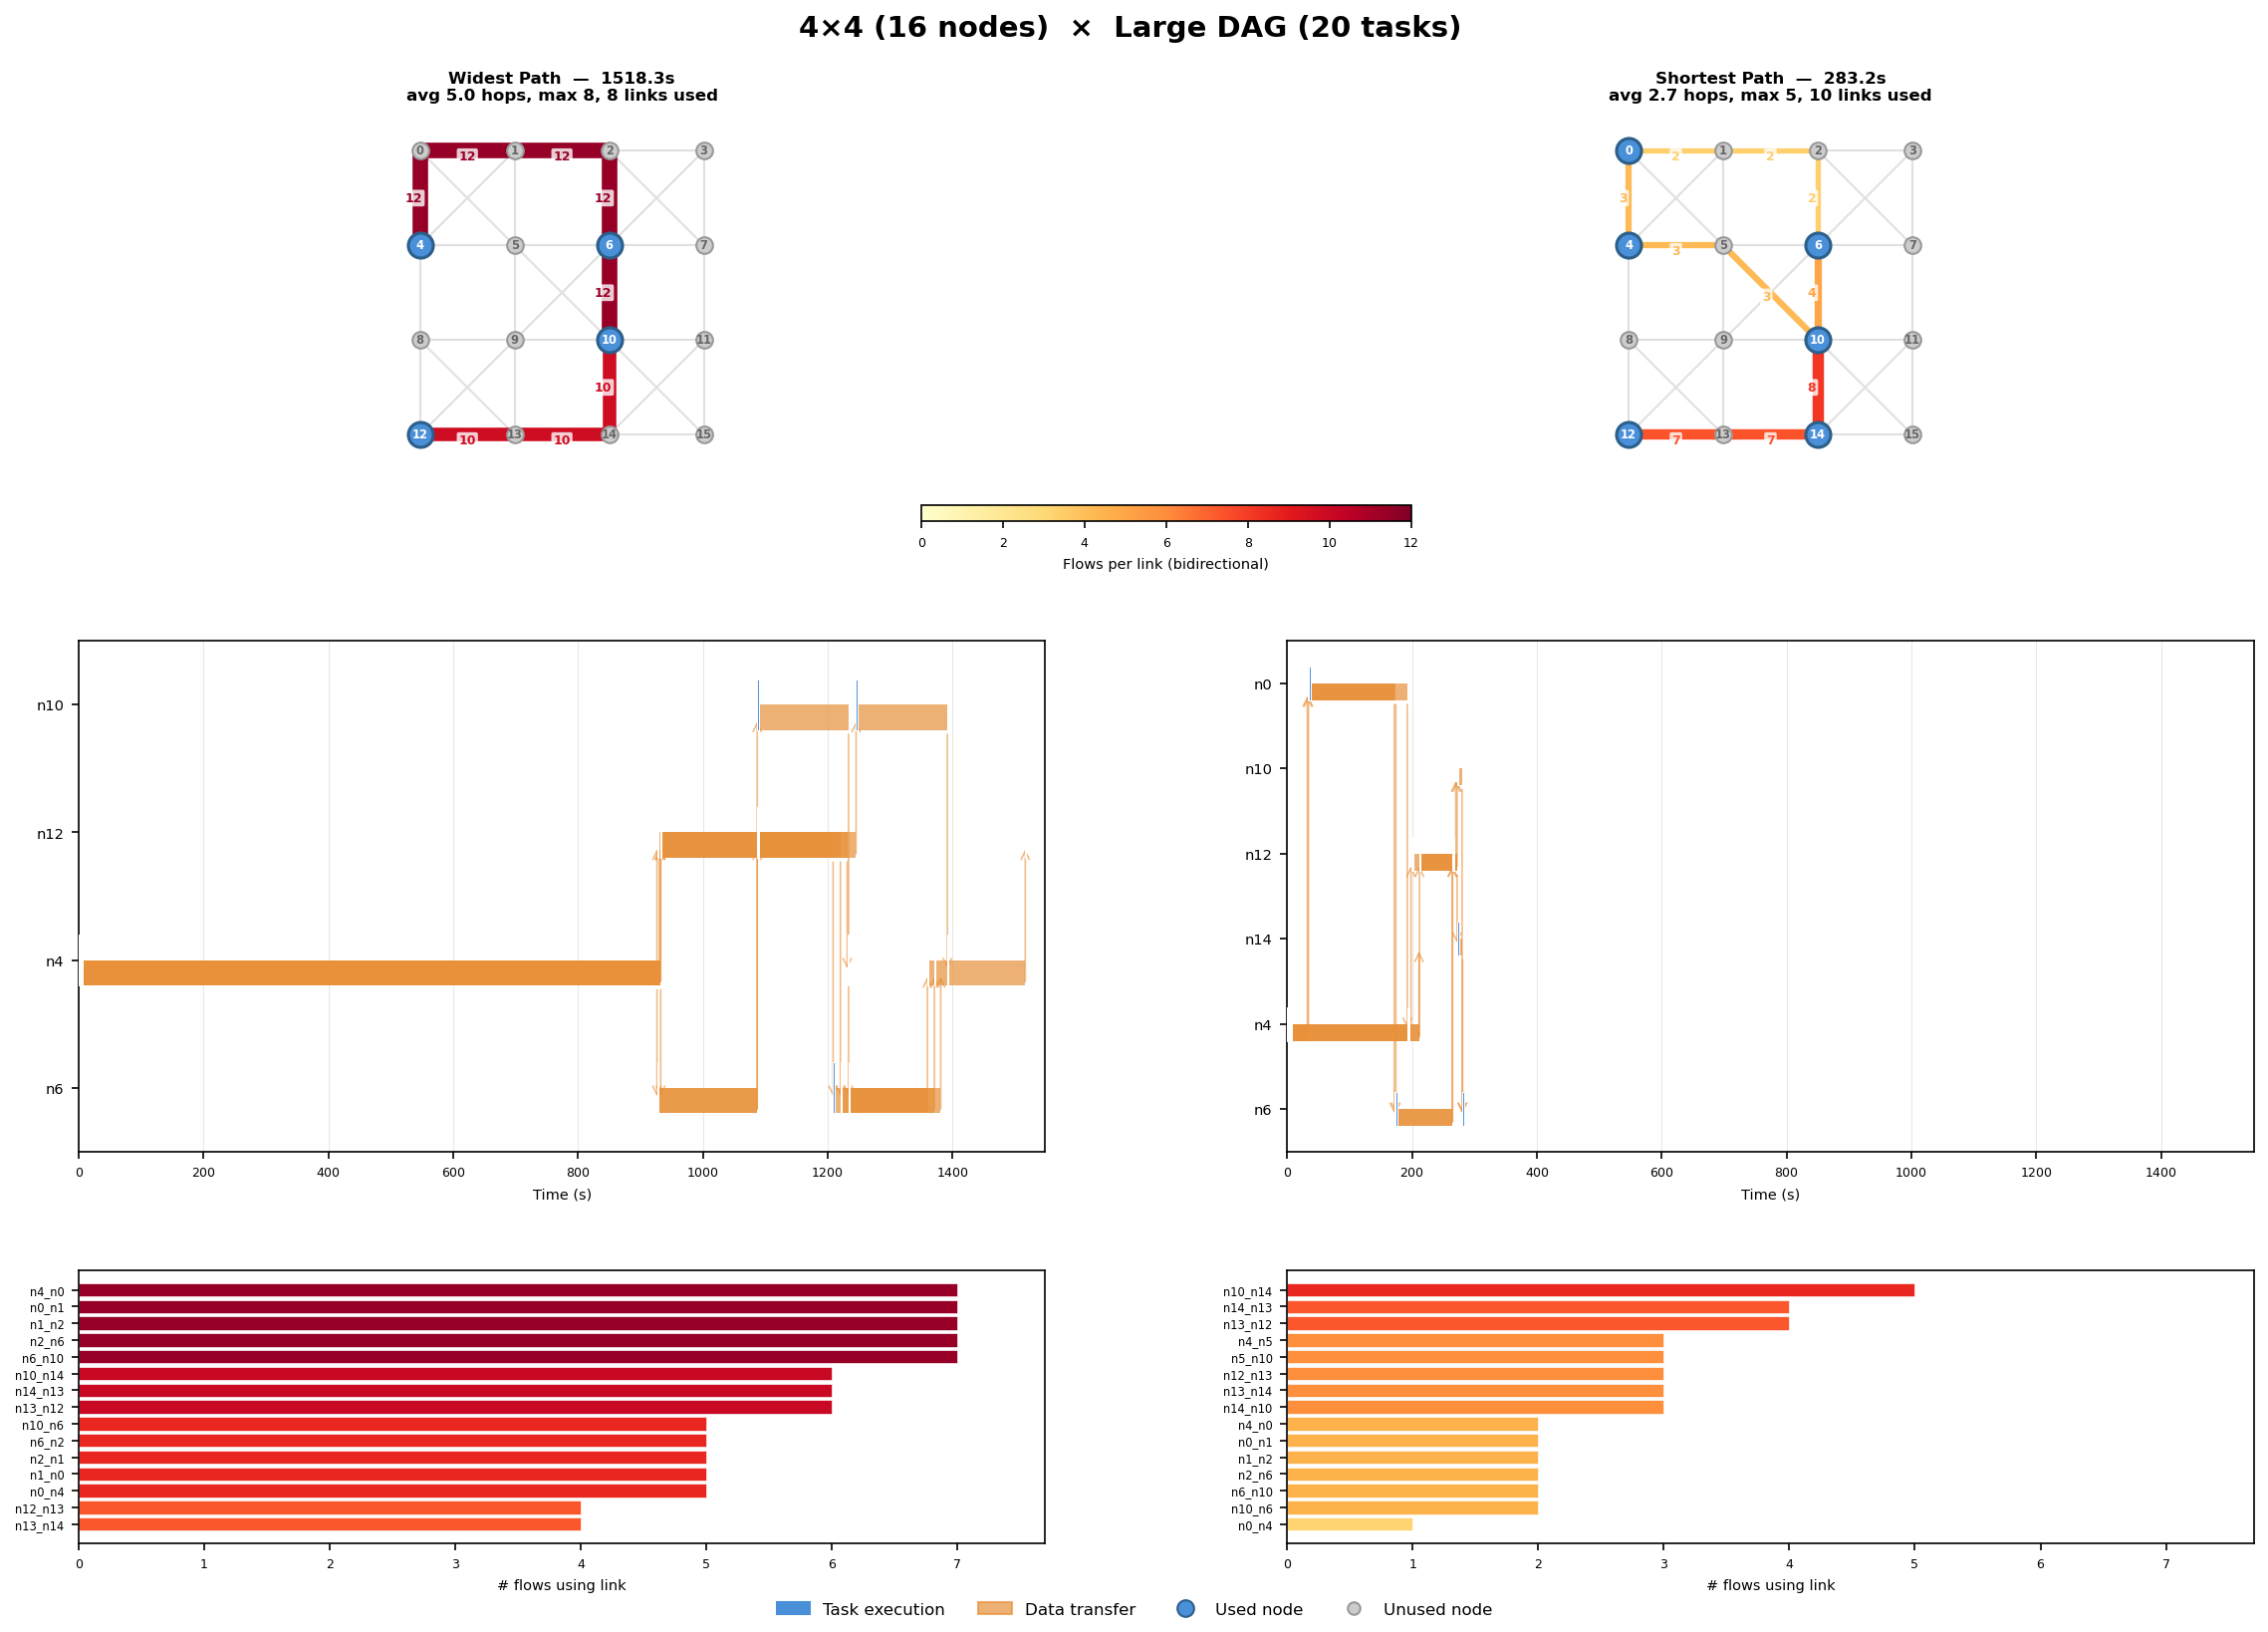
\includegraphics[width=\textwidth]{figures/largenet_largedag.png}
\caption{$4\times4$ $\times$ Large DAG. Widest path loads perimeter links with up to 12
bidirectional flows; shortest path distributes across the right side of the grid.}
\label{fig:ll}
\end{figure}

The worst case overall. Widest path routes 18 transfers through the perimeter,
loading n4$\to$n0 / n0$\to$n1 / n1$\to$n2 / n2$\to$n6 with
\textbf{7 flows each} (up to 12 bidirectional). The topology panel shows the
entire left and top edge as thick dark-red lines, while the right half of the
network is completely unused (gray). Average hop count is 5.0, max 8. The
first $\sim$925\,s is consumed entirely by outbound transfers. Shortest path
splits traffic across two paths on the right side of the grid
(n4$\to$n5$\to$n10$\to$n14 and n0$\to$n1$\to$n2$\to$n6), with max 5 flows
per link and avg 2.7 hops. Makespan: 1,518\,s vs.\ 283\,s ($5.4\times$
improvement).

%% ============================================================
\section{Discussion}

\subsection{Why Widest Path Fails Under CSMA}

Widest-path routing optimizes a \emph{single-flow} metric: it selects the path
with maximum bottleneck bandwidth. This is optimal when a single transfer uses
the network in isolation. However, DAG execution produces \emph{multiple
concurrent transfers}, and widest-path routing directs them all toward the
same high-bandwidth links. Under CSMA/Bianchi:

\begin{enumerate}
    \item \textbf{Flow concentration}: Multiple transfers share the same
    ``best'' links, dividing effective bandwidth by the number of concurrent
    flows via Bianchi MAC contention ($\eta(n)/n$ scales sublinearly).
    \item \textbf{Hop count inflation}: To reach distant high-bandwidth links,
    widest path takes longer routes. Each additional hop means one more link
    occupied simultaneously, increasing the total contention footprint.
    \item \textbf{Cascading delays}: Longer transfers block downstream tasks,
    pushing the critical path further out and amplifying the makespan.
\end{enumerate}

\subsection{When Widest Path Wins}

Widest path wins only in the $2\times2$ $\times$ Medium DAG case, where:
\begin{itemize}
    \item The network is so small that all paths have the same hop count (1 hop).
    \item Widest path's link preference happens to balance load across the
    two available physical links better than shortest path.
\end{itemize}
This is a degenerate case where the ``widest'' and ``shortest'' criteria
collapse to the same hop count, and the tiebreaking happens to favor balance.

\subsection{Scaling Behavior}

The widest-path penalty grows with both network size and DAG complexity:

\begin{itemize}
    \item \textbf{Network size}: Larger grids have longer ``widest'' routes
    (up to 8 hops on $4\times4$), amplifying the hop-count penalty.
    \item \textbf{DAG complexity}: More tasks produce more concurrent transfers,
    all competing for the same concentrated corridor.
\end{itemize}

On the $4\times4$ grid, widest path consistently produces makespans
$5$--$35\times$ longer than shortest path.

%% ============================================================
\section{Conclusion}

Under CSMA/Bianchi interference on wireless mesh networks, shortest-path
routing significantly outperforms widest-path routing for DAG-scheduled task
graphs. The key insight is that single-flow optimal routing (maximize
bottleneck bandwidth) becomes counterproductive when multiple flows compete
for shared wireless airtime. Shortest-path routing minimizes per-transfer link
occupancy, reduces the contention footprint, and distributes traffic across
more diverse paths. Future work could explore contention-aware routing that
jointly optimizes bandwidth and expected interference load.

\end{document}
